\documentclass{article}
% \VignettePackage{spca}
% \VignetteIndexEntry{A tutorial for spatial Analysis of Principal Components}

\usepackage{graphicx}
\usepackage[colorlinks=true,urlcolor=blue]{hyperref}
\usepackage{array}
\usepackage{color}
\usepackage{amsfonts}

\usepackage[utf8]{inputenc} % for UTF-8/single quotes from sQuote()


% for bold symbols in mathmode
\usepackage{bm}

\newcommand{\R}{\mathbb{R}}
\newcommand{\beq}{\begin{equation}}
\newcommand{\eeq}{\end{equation}}
\newcommand{\m}[1]{\mathbf{#1}}



\newcommand{\code}[1]{{{\tt #1}}}
\title{A tutorial for the spatial Analysis of Principal Components (sPCA) using \textit{adegenet} 1.3-0}
\author{Thibaut Jombart}
\date{\today}




\sloppy
\hyphenpenalty 10000


\usepackage{Sweave}
\begin{document}





\definecolor{Soutput}{rgb}{0,0,0.56}
\definecolor{Sinput}{rgb}{0.56,0,0}
\DefineVerbatimEnvironment{Sinput}{Verbatim}
{formatcom={\color{Sinput}},fontsize=\footnotesize, baselinestretch=0.75}
\DefineVerbatimEnvironment{Soutput}{Verbatim}
{formatcom={\color{Soutput}},fontsize=\footnotesize, baselinestretch=0.75}

\color{black}

\maketitle

\begin{abstract}
  This vignette provides a tutorial for the spatial analysis of principal components (sPCA, \cite{tjart04}) using
  the \textit{adegenet} package \cite{tjart05} for the R software \cite{np145}. sPCA is first
  illustrated using a simple simulated dataset, and then using empirical data of Chamois
  (\textit{Rupicapra rupicapra}) from the Bauges mountains (France). In particular, we illustrate
  how sPCA complements classical PCA by being more powerful for retrieving non-trivial spatial genetic patterns.
\end{abstract}


\newpage
\tableofcontents




\newpage
%%%%%%%%%%%%%%%%%%%%%%%%%%%
%%%%%%%%%%%%%%%%%%%%%%%%%%%
\section{Introduction}
%%%%%%%%%%%%%%%%%%%%%%%%%%%
%%%%%%%%%%%%%%%%%%%%%%%%%%%

This tutorial goes through the \emph{spatial Principal Component
  Analysis} (sPCA, \cite{tjart04}), a multivariate method devoted to
the identification of spatial genetic patterns.
The purpose of this tutorial is to provide guidelines for the application of sPCA as well as to
illustrate its usefulness for the investigation of spatial genetic patterns.
After briefly going through the rationale of the method, we introduce the different tools
implemented for sPCA in \textit{adegenet}.
This technical overview is then followed by the analysis of an empirical dataset which illustrates
the advantage of sPCA over classical PCA for investigating spatial patterns.




%%%%%%%%%%%%%%%%%%%%%%%%%%%
\subsection{Rationale of sPCA}
%%%%%%%%%%%%%%%%%%%%%%%%%%%
Mathematical notations used in this tutorial are identical to the original publication \cite{tjart04}.
The sPCA analyses a matrix of relative allele frequencies $\m{X}$ which contains genotypes or
populations (later refered to as 'entities') in rows and alleles in columns.
Spatial information is stored inside a spatial weighting matrix
$\m{L}$ which contains positive terms corresponding to some measurement
(often binary) of spatial proximity among entities.
Most often, these terms can be derived from a connection network built
upon a given algorithm (for instance, pp.572-576 in \cite{tj88}).
This matrix is row-standardized (\textit{i.e.}, each of its rows sums
to one), and all its diagonal terms are zero.
$\m{L}$ can be used to compute the spatial autocorrelation of a
given centred variable $\m{x}$ (\texttt{i.e.}, with mean zero) with $n$ observations ($\m{x} \in
\R^n$) using Moran's $I$ \cite{tj223,tj222,tj436}:
\beq
I(\m{x}) = \frac{\m{x}^T\m{Lx}}{\m{x}^T\m{x}}
\label{eqn:I}
\eeq

In the case of genetic data, $\m{x}$ contains frequencies of an allele.
Moran's $I$ can be used to measure spatial structure in the values
of $\m{x}$: it is highly positive when values of $\m{x}$ observed at
neighbouring sites tend to be similar (positive spatial
autocorrelation, referred to as \emph{global structures}), while it is
strongly negative when values of $\m{x}$ observed at
neighbouring sites tend to be dissimilar (negative spatial
autocorrelation, referred to as \emph{local structures}).
\\


However, since it is standardized by the variance of
$\m{x}$, Moran's index measures only spatial structures and not genetic variability.
The sPCA defines the following function to measure both spatial
structure and variability in $\m{x}$:
\beq
C(\m{x}) = \mbox{var}(\m{x})I(\m{x}) = \frac{1}{n}\m{x}^T\m{Lx}
\label{eqn:C}
\eeq

$C(\m{x})$ is highly positive when $\m{x}$ has a large variance and
exhibits a global structure; conversely, it is largely negative
when $\m{x}$ has a high variance and displays a local structure.
This function is the criterion used in sPCA, which finds linear
combinations of the alleles of $\m{X}$ (denoted $\m{Xv}$) decomposing $C$ from its
maximum to its minimum value.
Because $C(\m{Xv})$ is a product of variance and autocorrelation,
it is important, when interpreting the results, to detail both
components and to compare their value with their range of variation
(maximum attainable variance, as well as maximum and minimum $I$ are
known analytically).
A structure with a low spatial autocorrelation can barely be
interpreted as a spatial pattern; similarly, a structure with a low
variance would likely not reflect any genetic structure.
We will later see how these information can be retrieved from \texttt{spca} results.





%%%%%%%%%%%%%%%%%%%%%%%%%%%
\subsection{The \texttt{spca} function}
%%%%%%%%%%%%%%%%%%%%%%%%%%%
The simulated dataset used to illustrate this section has been
analyzed in \cite{tjart04}, and corresponds to Figure 2A of the article.
In \textit{adegenet}, the matrix of alleles frequencies previously
denoted $\m{X}$ exactly corresponds to the \texttt{@tab} slot of \texttt{genind} or
\texttt{genpop} objects:
\begin{Schunk}
\begin{Sinput}
> library(adegenet)
> library(adehabitat)
> data(spcaIllus)
> obj <- spcaIllus$dat2A
> obj
\end{Sinput}
\begin{Soutput}
   #####################
   ### Genind object ### 
   #####################
- genotypes of individuals - 

S4 class:  genind
@call: old2new(object = obj)

@tab:  80 x 192 matrix of genotypes

@ind.names: vector of  80 individual names
@loc.names: vector of  20 locus names
@loc.nall: number of alleles per locus
@loc.fac: locus factor for the  192 columns of @tab
@all.names: list of  20 components yielding allele names for each locus
@ploidy:  2
@type:  codom

Optionnal contents: 
@pop:  factor giving the population of each individual
@pop.names:  factor giving the population of each individual

@other: a list containing: xy 
\end{Soutput}
\begin{Sinput}
> head(truenames(obj[loc = "L01"])$tab)
\end{Sinput}
\begin{Soutput}
     L01.1 L01.2 L01.3 L01.4 L01.5 L01.6 L01.7 L01.8 L01.9
0035     0     0   0.0     0   0.5   0.5     0   0.0   0.0
0352     0     0   0.5     0   0.5   0.0     0   0.0   0.0
0423     0     0   0.0     0   0.5   0.0     0   0.0   0.5
0289     0     0   0.0     0   0.0   0.5     0   0.0   0.5
0487     0     0   0.0     0   0.0   0.5     0   0.5   0.0
0053     0     0   0.0     0   0.5   0.5     0   0.0   0.0
\end{Soutput}
\end{Schunk}
\noindent The object \texttt{obj} is a \texttt{genind} object; note
that here, we only displayed the table for the first locus (\texttt{loc="L01"}).
\\


The function performing the sPCA is \texttt{spca}; it accepts a bunch
of arguments, but only the first two are mandatory to perform the
analysis (see \texttt{?spca} for further information):
\begin{Schunk}
\begin{Sinput}
> args(spca)
\end{Sinput}
\begin{Soutput}
function (obj, xy = NULL, cn = NULL, matWeight = NULL, scale = FALSE, 
    scale.method = c("sigma", "binom"), scannf = TRUE, nfposi = 1, 
    nfnega = 1, type = NULL, ask = TRUE, plot.nb = TRUE, edit.nb = FALSE, 
    truenames = TRUE, d1 = NULL, d2 = NULL, k = NULL, a = NULL, 
    dmin = NULL) 
NULL
\end{Soutput}
\end{Schunk}
The argument \texttt{obj} is a \texttt{genind}/\texttt{genpop} object.
By definition in sPCA, the studied entities are georeferenced.
The spatial information can be provided to the function \texttt{spca}
in several ways, the first being through the \texttt{xy} argument,
which is a matrix of spatial coordinates with
'x' and 'y' coordinates in columns.
Alternatively, these coordinates can be stored inside the
\texttt{genind}/\texttt{genpop} object, preferably as
\texttt{@other\$xy}, in which case the \texttt{spca} function will detect and use this information,
and not
request an \texttt{xy} argument.
Note that \texttt{obj} already contains spatial coordinates at the
appropriate place.
Hence, we can use the following command to run the sPCA (\texttt{ask} and \texttt{scannf}
are set to FALSE to avoid interactivity):
\begin{Schunk}
\begin{Sinput}
> mySpca <- spca(obj, ask = FALSE, type = 1, scannf = FALSE)
\end{Sinput}
\end{Schunk}
~\\


Note, however, that spatial coordinates are not directly used in sPCA:
the spatial information is included in the analysis by the spatial
weighting matrix $\m{L}$ derived from a connection network (eq. \ref{eqn:I} and \ref{eqn:C}).
Technically, the \texttt{spca} function can incorporate spatial weightings as a matrix (argument
\texttt{matWeight}), as a connection network with the classes
\texttt{nb} or \texttt{listw} (argument \texttt{cn}), both implemented in the \texttt{spdep} package.
The function \texttt{chooseCN} is a wrapper for different functions
scattered across several packages implementing a variety of connection networks.
If only spatial coordinates are provided to \texttt{spca},
\texttt{chooseCN} is called to construct an appropriate graph.
See \texttt{?chooseCN} for more information.
Note that many of the \texttt{spca} arguments are in fact arguments
for \texttt{chooseCN}: \texttt{type}, \texttt{ask}, \texttt{plot.nb},
\texttt{edit.nb}, \texttt{d1}, \texttt{d2}, \texttt{k}, \texttt{a}, and \texttt{dmin}.
For instance, the command:
\begin{Schunk}
\begin{Sinput}
> mySpca <- spca(obj, type = 1, ask = FALSE, scannf = FALSE)
\end{Sinput}
\end{Schunk}
\noindent performs a sPCA using the Delaunay triangulation as
connection network (\texttt{type=1}, see \texttt{?chooseCN}), while
the command:
\begin{Schunk}
\begin{Sinput}
> mySpca <- spca(obj, type = 5, d1 = 0, d2 = 2, scannf = FALSE)
\end{Sinput}
\end{Schunk}
\noindent computes a sPCA using a connection network which defines
neighbouring entities based on pairwise geographic distances (\texttt{type=5}),
considering as neighbours two entities whose distance between 0 (\texttt{d1=0}) and 2 (\texttt{d2=2}).
\\


Another possibility is of course to provide directly a connection
network (\texttt{nb} object) or a list of spatial weights
(\texttt{listw} object) to the \texttt{spca} function; this can be done via the \texttt{cn} argument.
For instance:
\begin{Schunk}
\begin{Sinput}
> myCn <- chooseCN(obj$other$xy, type = 6, k = 10, plot = FALSE)
> myCn
\end{Sinput}
\begin{Soutput}
Neighbour list object:
Number of regions: 80 
Number of nonzero links: 932 
Percentage nonzero weights: 14.5625 
Average number of links: 11.65 
\end{Soutput}
\begin{Sinput}
> class(myCn)
\end{Sinput}
\begin{Soutput}
[1] "nb"
\end{Soutput}
\begin{Sinput}
> mySpca2 <- spca(obj, cn = myCn, scannf = FALSE)
\end{Sinput}
\end{Schunk}
\noindent produces a sPCA using \texttt{myCn} ($k=10$ nearest
neighbours) as a connection network.
\\


When used interactively (\texttt{scannf=TRUE}), \texttt{spca} displays a barplot of eigenvalues and
asks the user for a number of positive axes ('first number of axes') and negative
axes ('second number of axes') to be retained.
For the object \texttt{mySpca}, this barplot would be (here we
indicate in red the retained eigenvalue):
\begin{Schunk}
\begin{Sinput}
> barplot(mySpca$eig, main = "Eigenvalues of sPCA", col = rep(c("red", 
+     "grey"), c(1, 100)))
\end{Sinput}
\end{Schunk}
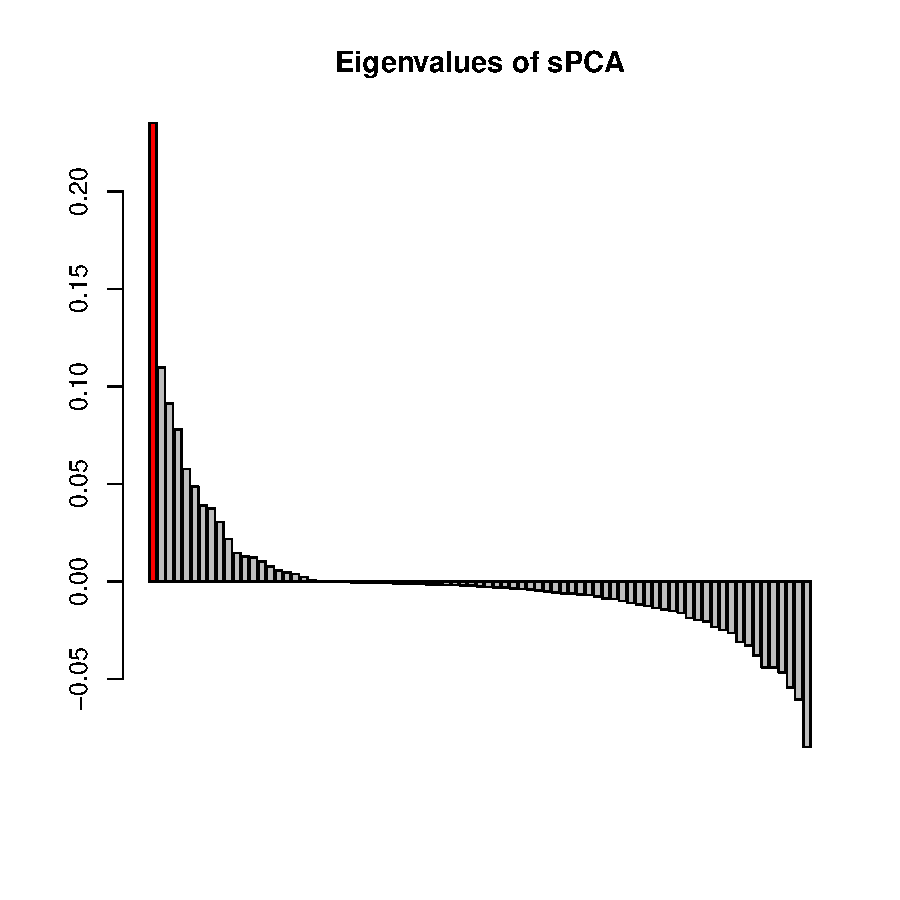
\includegraphics{figs/spca-009}

\noindent Positive eigenvalues (on the left) correspond to global
structures, while negative eigenvalues (on the right) indicate local patterns.
Actual structures should result in more extreme (positive or
negative) eigenvalues; for instance, the object \texttt{mySpca} likely
contains one single global structure, and no local structure.
If one does not want to choose the number of retained axes
interactively, the arguments \texttt{nfposi} (number of retained
factors with positive eigenvalues) and \texttt{nfnega} (number of
retained factors with negative eigenvalues) can be used.
Once this information has been provided to \texttt{spca}, the
analysis is computed and stored inside an object with the class \texttt{spca}.





%%%%%%%%%%%%%%%%%%%%%%%%%%%
\subsection{Contents of a \texttt{spca} object}
%%%%%%%%%%%%%%%%%%%%%%%%%%%
Let us consider a \texttt{spca} object resulting from the analysis of
the object \texttt{obj}, using a Delaunay triangulation (\texttt{type=1}) as connection network:
\begin{Schunk}
\begin{Sinput}
> mySpca <- spca(obj, type = 1, scannf = FALSE, plot.nb = FALSE, 
+     nfposi = 1, nfnega = 0)
> class(mySpca)
\end{Sinput}
\begin{Soutput}
[1] "spca"
\end{Soutput}
\begin{Sinput}
> mySpca
\end{Sinput}
\begin{Soutput}
	########################################
	# spatial Principal Component Analysis #
	########################################
class: spca
$call: spca(obj = obj, scannf = FALSE, nfposi = 1, nfnega = 0, type = 1, 
    plot.nb = FALSE)

$nfposi: 1 axis-components saved
$nfnega: 0 axis-components saved
Positive eigenvalues: 0.2309 0.1118 0.09379 0.07817 0.06911 ...
Negative eigenvalues: -0.08421 -0.07376 -0.06978 -0.06648 -0.06279 ...

  vector length mode    content    
1 $eig   79     numeric eigenvalues

  data.frame nrow ncol content                                                 
1 $c1        192  1    principal axes: scaled vectors of alleles loadings      
2 $li        80   1    principal components: coordinates of entities ('scores')
3 $ls        80   1    lag vector of principal components                      
4 $as        2    1    pca axes onto spca axes                                 

$xy: matrix of spatial coordinates
$lw: a list of spatial weights (class 'listw')

other elements: NULL
\end{Soutput}
\end{Schunk}

\noindent An \texttt{spca} object is a list containing all required
information about a performed sPCA.
Details about the different components of such a list can be found in
the \texttt{spca} documentation (\texttt{?spca}).
The purpose of this section is to explicit how the elements described
in \cite{tjart04} are stored inside a \texttt{spca} object.

First, eigenvalues of the analysis are stored inside the
\texttt{\$eig} component as a numeric vector stored in decreasing order:
\begin{Schunk}
\begin{Sinput}
> head(mySpca$eig)
\end{Sinput}
\begin{Soutput}
[1] 0.23087862 0.11184721 0.09378750 0.07816561 0.06910536 0.06429596
\end{Soutput}
\begin{Sinput}
> tail(mySpca$eig)
\end{Sinput}
\begin{Soutput}
[1] -0.05480010 -0.06279067 -0.06647896 -0.06978457 -0.07375563 -0.08421213
\end{Soutput}
\begin{Sinput}
> length(mySpca$eig)
\end{Sinput}
\begin{Soutput}
[1] 79
\end{Soutput}
\begin{Sinput}
> myPal <- colorRampPalette(c("red", "grey", "blue"))
> barplot(mySpca$eig, main = "A variant of the plot\n of sPCA eigenvalues", 
+     col = myPal(length(mySpca$eig)))
> legend("topright", fill = c("red", "blue"), leg = c("Global structures", 
+     "Local structures"))
> abline(h = 0, col = "grey")
\end{Sinput}
\end{Schunk}
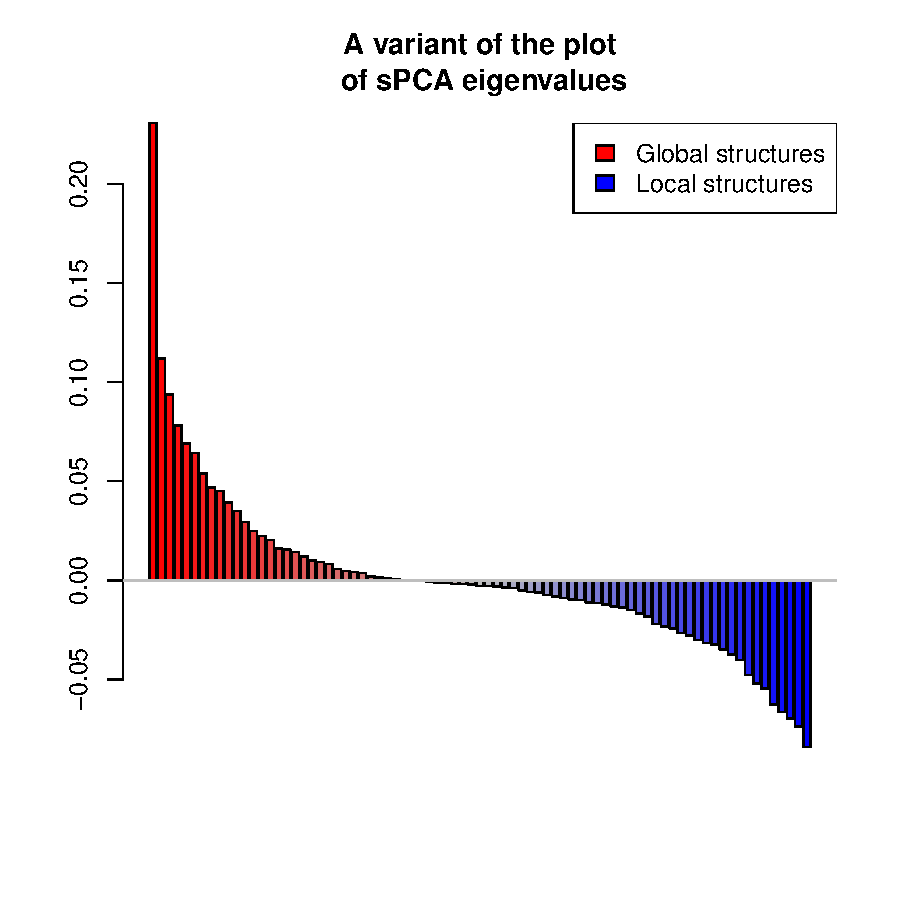
\includegraphics{figs/spca-011}

\noindent The axes of the analysis, denoted $\m{v}$ in eq. (4) \cite{tjart04}
are stored as columns inside the \texttt{\$c1} component.
Each column contains loadings for all the alleles:
\begin{Schunk}
\begin{Sinput}
> head(mySpca$c1)
\end{Sinput}
\begin{Soutput}
             Axis 1
L01.1  1.268838e-02
L01.2  2.220446e-16
L01.3 -1.119979e-01
L01.4 -4.440892e-16
L01.5 -2.766095e-02
L01.6 -4.477031e-02
\end{Soutput}
\begin{Sinput}
> tail(mySpca$c1)
\end{Sinput}
\begin{Soutput}
           Axis 1
L20.3  0.28715850
L20.4  0.01485180
L20.5 -0.01500353
L20.6  0.01659481
L20.7 -0.14260743
L20.8 -0.15388988
\end{Soutput}
\begin{Sinput}
> dim(mySpca$c1)
\end{Sinput}
\begin{Soutput}
[1] 192   1
\end{Soutput}
\end{Schunk}


\noindent The entity scores, denoted $\psi = \m{Xv}$ in the article, are stored
in columns in the \texttt{\$li} component:
\begin{Schunk}
\begin{Sinput}
> head(mySpca$li)
\end{Sinput}
\begin{Soutput}
         Axis 1
0035 -0.4367748
0352 -0.8052723
0423 -0.4337114
0289  0.1434650
0487 -0.4802931
0053 -0.5421831
\end{Soutput}
\begin{Sinput}
> tail(mySpca$li)
\end{Sinput}
\begin{Soutput}
          Axis 1
1074 -0.06178196
1187 -0.08144162
1260  0.41491795
1038  0.25643986
1434  0.35618737
1218  0.21433977
\end{Soutput}
\begin{Sinput}
> dim(mySpca$li)
\end{Sinput}
\begin{Soutput}
[1] 80  1
\end{Soutput}
\end{Schunk}

\noindent The lag vectors of the scores can be used to better perceive
global structures.
Lag vectors are stored in the \texttt{\$ls} component:
\begin{Schunk}
\begin{Sinput}
> head(mySpca$ls)
\end{Sinput}
\begin{Soutput}
         Axis 1
0035 -0.7076732
0352 -0.6321654
0423 -0.4822952
0289  0.3947791
0487 -0.2803381
0053 -0.4848376
\end{Soutput}
\begin{Sinput}
> tail(mySpca$ls)
\end{Sinput}
\begin{Soutput}
         Axis 1
1074  0.4930238
1187 -0.8384871
1260  0.6887072
1038  0.3665794
1434  0.3109197
1218  0.3329688
\end{Soutput}
\begin{Sinput}
> dim(mySpca$ls)
\end{Sinput}
\begin{Soutput}
[1] 80  1
\end{Soutput}
\end{Schunk}

\noindent Lastly, we can compare the axes of an classical
PCA (denoted $\m{u}$ in the paper) to the axes of the sPCA ($\m{v}$).
This is achieved by projecting $\m{u}$ onto $\m{v}$, but this
projection is a particular one: because both $\m{u}$ and $\m{v}$ are
centred to mean zero and scaled to unit variance, the value of the
projection simply is the correlation between both axes.
This information is stored inside the \texttt{\$as} component:
\begin{Schunk}
\begin{Sinput}
> mySpca$as
\end{Sinput}
\begin{Soutput}
              Axis 1
PCA Axis1 -0.7363595
PCA Axis2  0.3395674
\end{Soutput}
\end{Schunk}





%%%%%%%%%%%%%%%%%%%%%%%%%%%
\subsection{Graphical display of \texttt{spca} results}
%%%%%%%%%%%%%%%%%%%%%%%%%%%

The information contained inside a \texttt{spca} object can be displayed
in several ways.
While we have seen that a simple barplot of sPCA eigenvalues can give a first idea of the
global and local structures to be retained, we have also seen that
each eigenvalue can be decomposed into a \textit{variance} and a
\textit{spatial autocorrelation} (Moran's $I$) component.
This information is provided by the \texttt{summary} function, but it
can also be represented graphically.
The corresponding function is \texttt{screeplot}, and can be used on any
\texttt{spca} object:
\begin{Schunk}
\begin{Sinput}
> screeplot(mySpca)
\end{Sinput}
\end{Schunk}
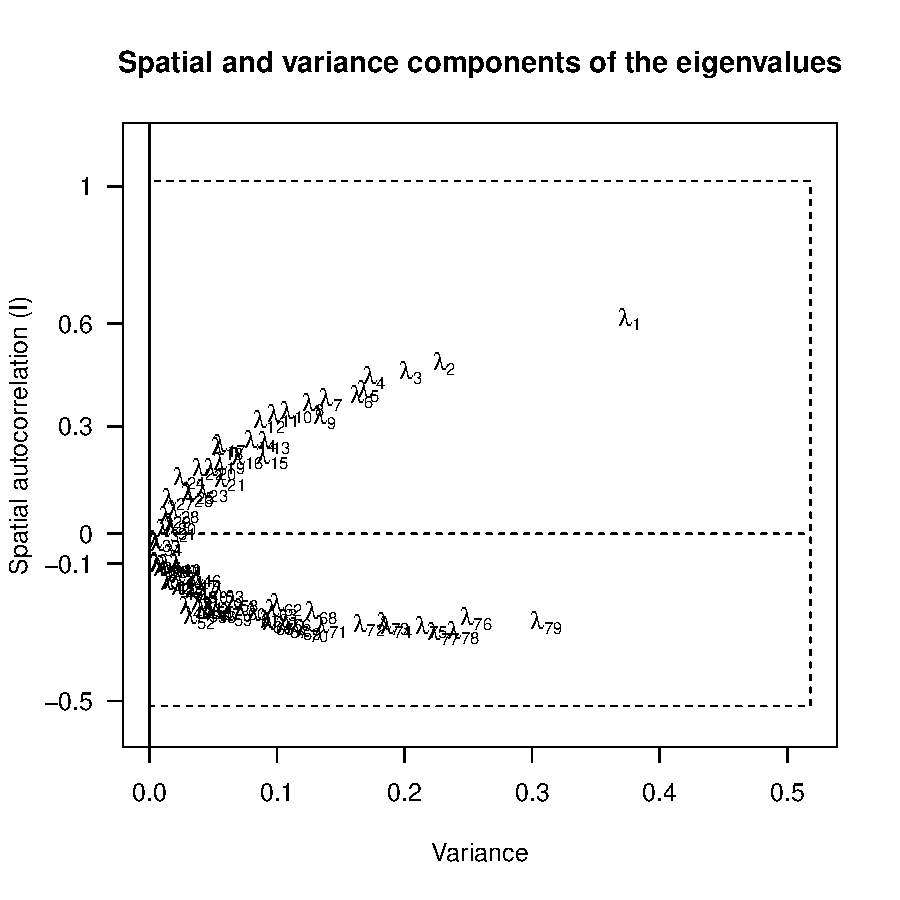
\includegraphics{figs/spca-screeplot}

\noindent The resulting figure represents eigenvalues of sPCA (denoted
$\lambda_i$ with $i=1,\ldots,r$, where $\lambda_1$ is the highest
positive eigenvalue, and $\lambda_{r}$ is the highest negative
eigenvalue) according the their variance and Moran's $I$ components.
These eigenvalues are contained inside a rectangle indicated in dashed
lines.
The maximum attainable variance by a linear combination of alleles is
the one from an ordinary PCA, indicated by the vertical dashed line on
the right.
The two horizontal dashed lines indicate the range of variation of
Moran's $I$, given the spatial weighting matrix that was used.
This figure is useful to assess whether a given score of entities contains
relatively enough variability and spatial structuring to be interpreted.
For instance, here, $\lambda_1$ clearly is the largest eigenvalue in
terms of variance and of spatial autocorrelation, and can be well
distinguished from all the other eigenvalues.
Hence, only the first global structure, associated to $\lambda_1$, should be interpreted.
\\


The global and local tests proposed in \cite{tjart04} can
be used to reinforce the decision of interpreting or not
interpreting global and local structures.
Each test can detect the presence of one kind of structure.
We can apply them to the object \texttt{obj}, used in our sPCA:
\begin{Schunk}
\begin{Sinput}
> myGtest <- global.rtest(obj$tab, mySpca$lw, nperm = 99)
> myGtest
\end{Sinput}
\begin{Soutput}
Monte-Carlo test
Call: global.rtest(X = obj$tab, listw = mySpca$lw, nperm = 99)

Observation: 0.01658103 

Based on 99 replicates
Simulated p-value: 0.01 
Alternative hypothesis: greater 

     Std.Obs  Expectation     Variance 
3.986172e+00 1.289255e-02 8.562127e-07 
\end{Soutput}
\begin{Sinput}
> plot(myGtest)
\end{Sinput}
\end{Schunk}
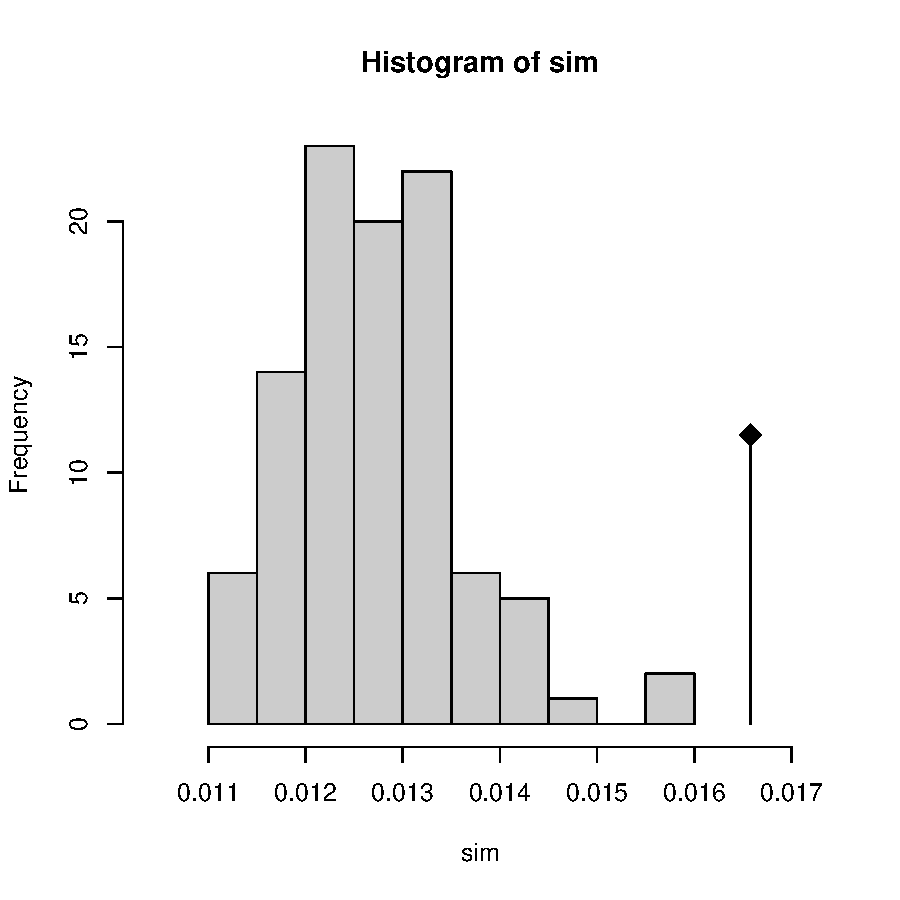
\includegraphics{figs/spca-globalrtest}

\noindent The produced object is a \texttt{randtest} object (see
\texttt{?randtest}), which is the class of objects for Monte-Carlo
tests in the \textit{ade4} package.
As shown, such object can be plotted using a \texttt{plot} function:
the resulting figure shows an histogram of permuted test statistics
and indicates the observed statistics by a black dot and a segment.
Here, the plot clearly shows that the oberved test statistic is larger
than most simulated values, leading to a likely rejection of
the null hypothesis of absence of spatial structure.
Note that because 99 permutations were used, the p-value cannot be
lower than 0.01.
In practice, more permutations should be used (like 999 or 9999 for results
intended to be published).

The same can be done with the local test, which here we do not expect
to be significant:
\begin{Schunk}
\begin{Sinput}
> myLtest <- local.rtest(obj$tab, mySpca$lw, nperm = 99)
> myLtest
\end{Sinput}
\begin{Soutput}
Monte-Carlo test
Call: local.rtest(X = obj$tab, listw = mySpca$lw, nperm = 99)

Observation: 0.01397349 

Based on 99 replicates
Simulated p-value: 0.18 
Alternative hypothesis: greater 

     Std.Obs  Expectation     Variance 
8.138443e-01 1.329193e-02 7.013349e-07 
\end{Soutput}
\begin{Sinput}
> plot(myLtest)
\end{Sinput}
\end{Schunk}
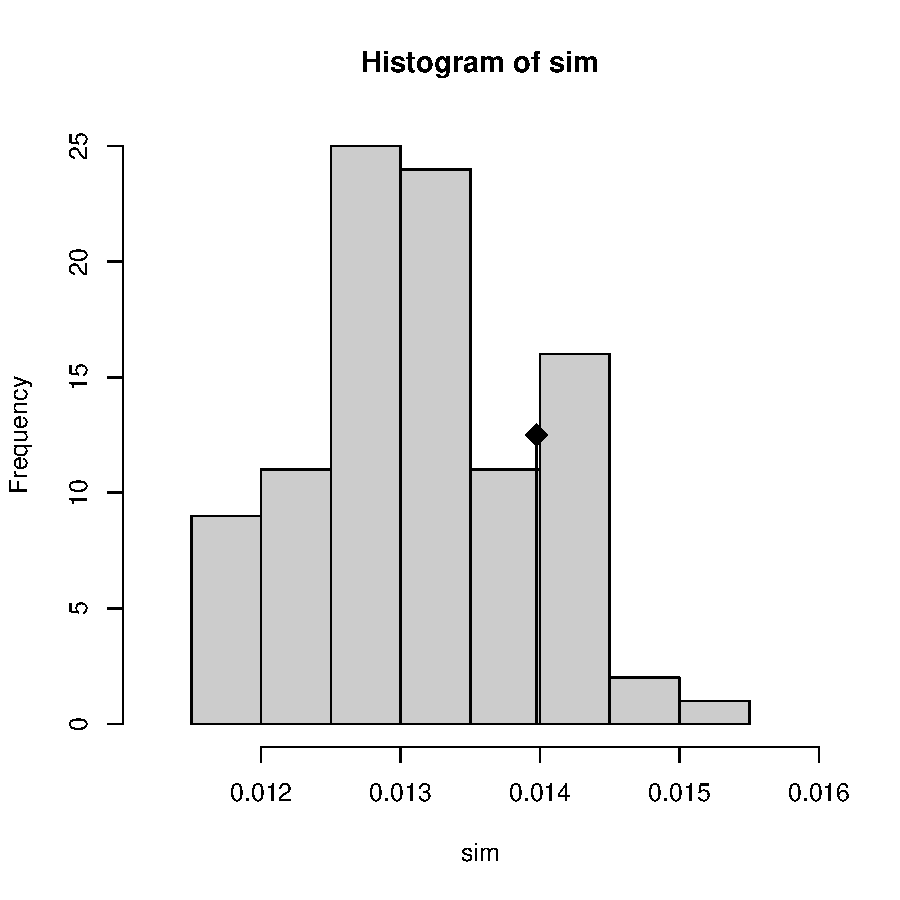
\includegraphics{figs/spca-localrtest}
~\\


Once we have an idea of which structures shall be interpreted, we can
try to visualize spatial genetic patterns.
There are several ways to do so.
The first, most simple approach is through the function plot (see \texttt{?plot.spca}):
\begin{Schunk}
\begin{Sinput}
> plot(mySpca)
\end{Sinput}
\end{Schunk}
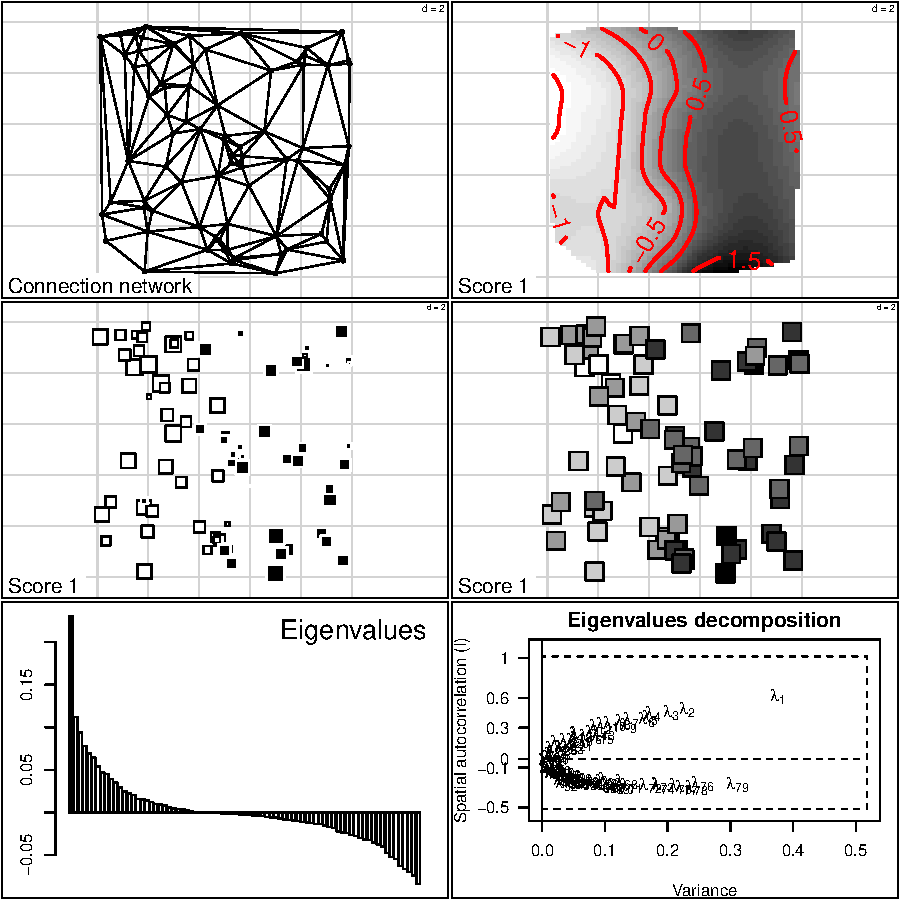
\includegraphics{figs/spca-plotspca}


\noindent This figure displays various information, that we detail from
the top to bottom and from left to right (also see \texttt{?plot.spca}).
The first plot shows the connection network that was used to define
spatial weightings.
The second, third, and fourth plots are different representations of
a score of entities in space, the first global score being the default (argument
\texttt{axis}).
In each, the values of scores (\texttt{\$li[,axis]} component of the
\texttt{spca} object) are represented using black and white symbols
(a variant being grey levels): white for negative values, and black
for positive values.
The second plot is a local interpolation of scores (function
\texttt{s.image} in \textit{ade4}), using grey levels, with contour lines.
The closer the contour lines are from each other, the stepest the
genetic differentiation is.
The third plot uses different sizes of squares to represent different
absolute values (\texttt{s.value} in \textit{ade4}): large black squares are well differentiated from
large white squares, but small squares are less differentiated.
The fourth plot is a variant using grey levels (\texttt{s.value} in
\textit{ade4}, with 'greylevel' method).
Here, all the three representations of the first global score show
that genotypes are splitted in two genetical clusters, one in the west
(or left) and one in the east (right).
The last two plots of the \texttt{plot.spca} function are the two
already seen displays of eigenvalues.
\\


While the default \texttt{plot} function for \texttt{spca} objects provides a useful summary of the
results, more flexible tools are needed e.g. to map the principal components onto the geographic space.
This can be achieved using the
\texttt{colorplot} function.
This function can summarize up to three scores at the same time by
translating each score into a channel of color (red, green, and blue).
The obtained values are used to compose a color using the RGB system.
See \texttt{?colorplot} for details about this function.
The original idea of such representation is due to \cite{tj179}.
Despite the \texttt{colorplot} clearly is more powerful to represent
more than one score on a single map, we can use it to represent the
first global structure that was retained in \texttt{mySpca}:
\begin{Schunk}
\begin{Sinput}
> colorplot(mySpca, cex = 3, main = "colorplot of mySpca, first global score")
\end{Sinput}
\end{Schunk}
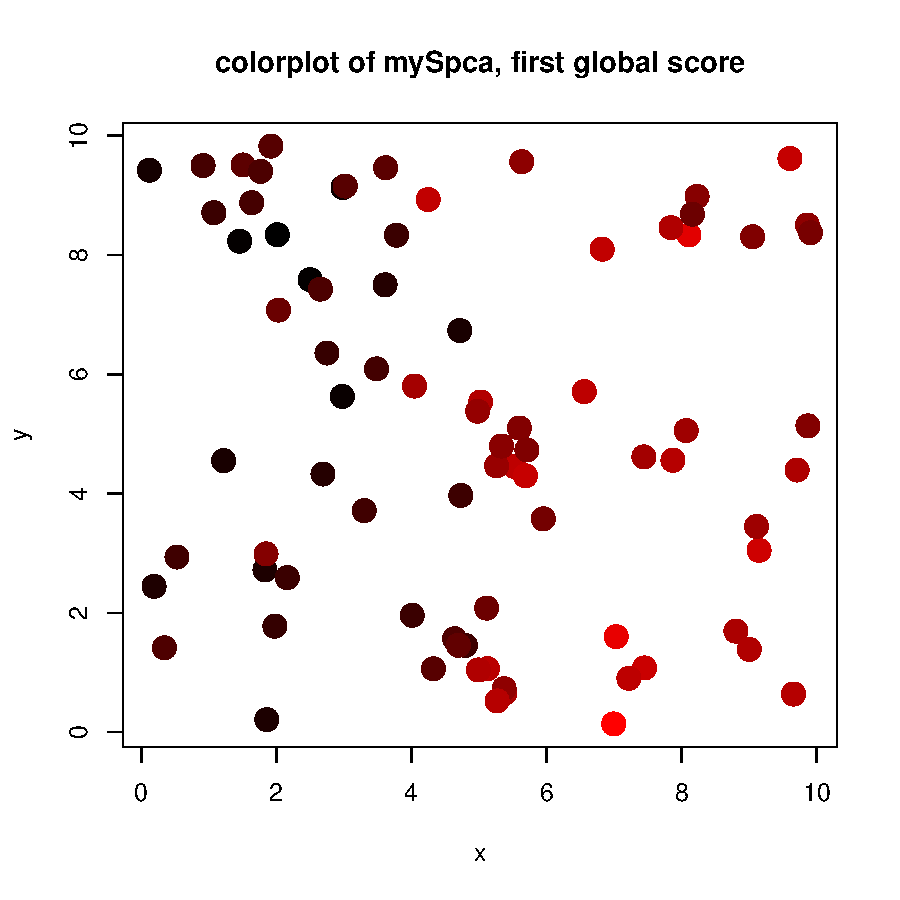
\includegraphics{figs/spca-colorplot}

\noindent See examples in \texttt{?colorplot} and \texttt{?spca}
for more examples of applications of colorplot to represent sPCA scores.
\\

Another common practice is interpolating principal components to get maps of genetic clines.
Note that it is crucial to perform this interpolation after the analysis, and not before, which
would add artefactual structures to the data.
Interpolation is easy to realize using \texttt{interp} from the \texttt{akima} package, and
\texttt{image}, or \texttt{filled.contour} to display the results:
\begin{Schunk}
\begin{Sinput}
> library(akima)
> x <- other(obj)$xy[, 1]
> y <- other(obj)$xy[, 2]
\end{Sinput}
\end{Schunk}
\begin{Schunk}
\begin{Sinput}
> temp <- interp(x, y, mySpca$li[, 1])
> image(temp)
\end{Sinput}
\end{Schunk}
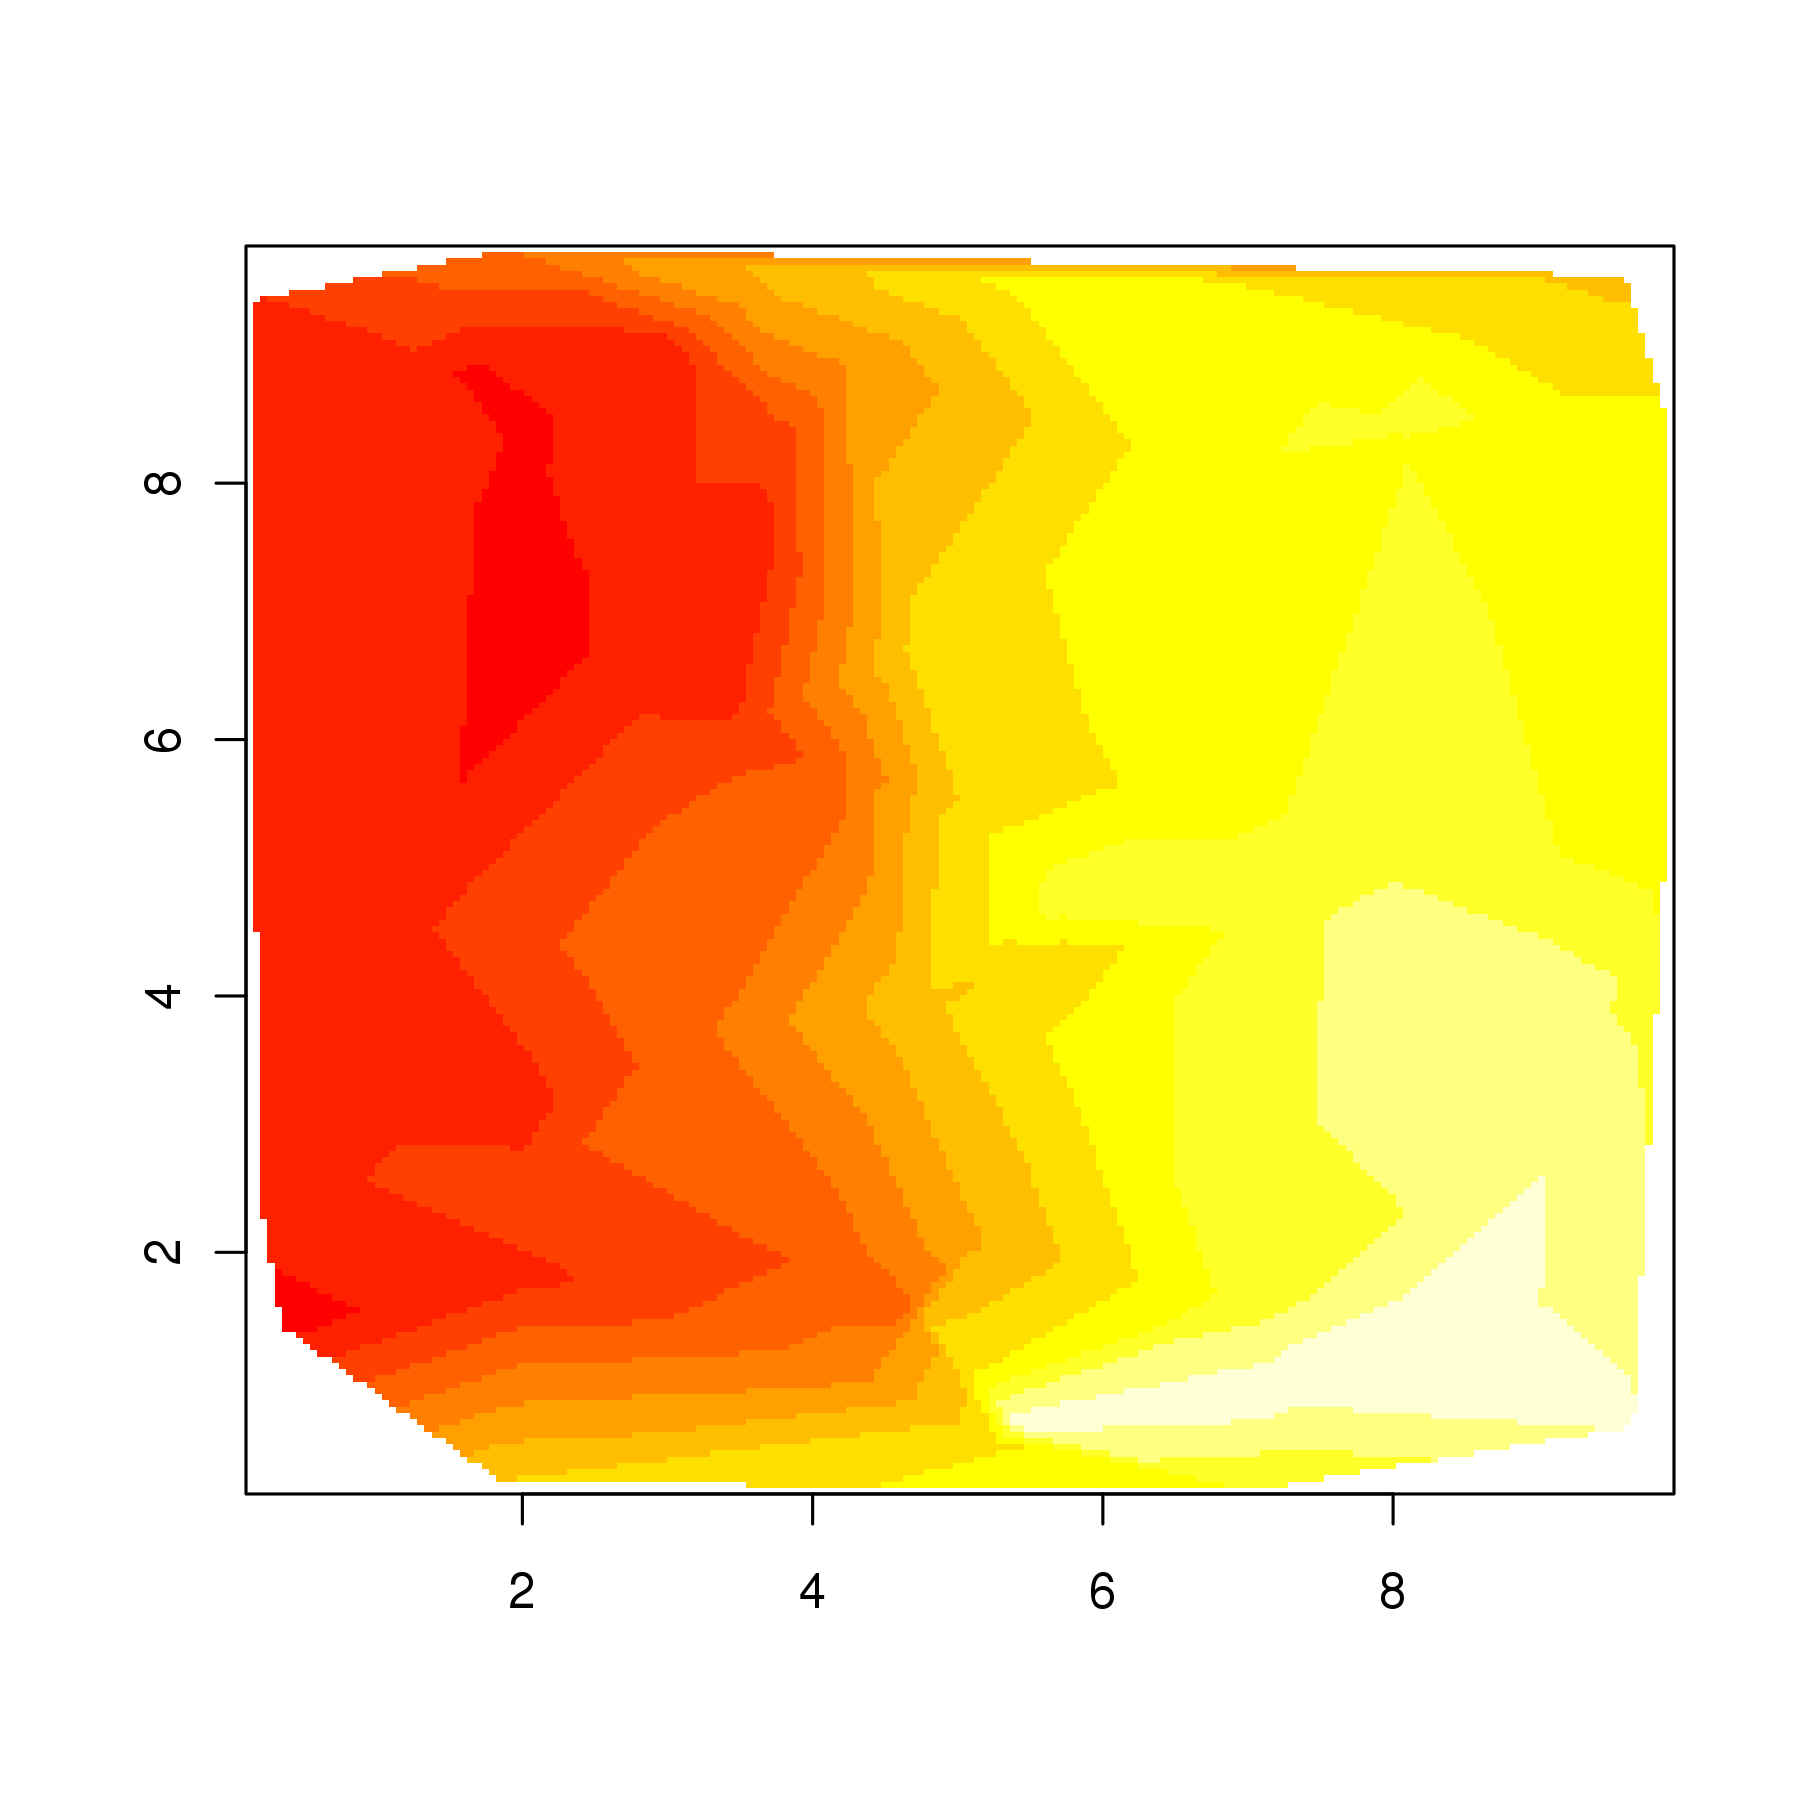
\includegraphics{figs/spca-022}

\noindent Note that for better clarity, we can use the lagged principal scores (\texttt{\$ls})
rather than the original scores (\texttt{\$li}); we also achieve a better resolution using specific
interpolated coordinates:
\begin{Schunk}
\begin{Sinput}
> interpX <- seq(min(x), max(x), le = 200)
> interpY <- seq(min(y), max(y), le = 200)
> temp <- interp(x, y, mySpca$ls[, 1], xo = interpX, yo = interpY)
> image(temp)
\end{Sinput}
\end{Schunk}
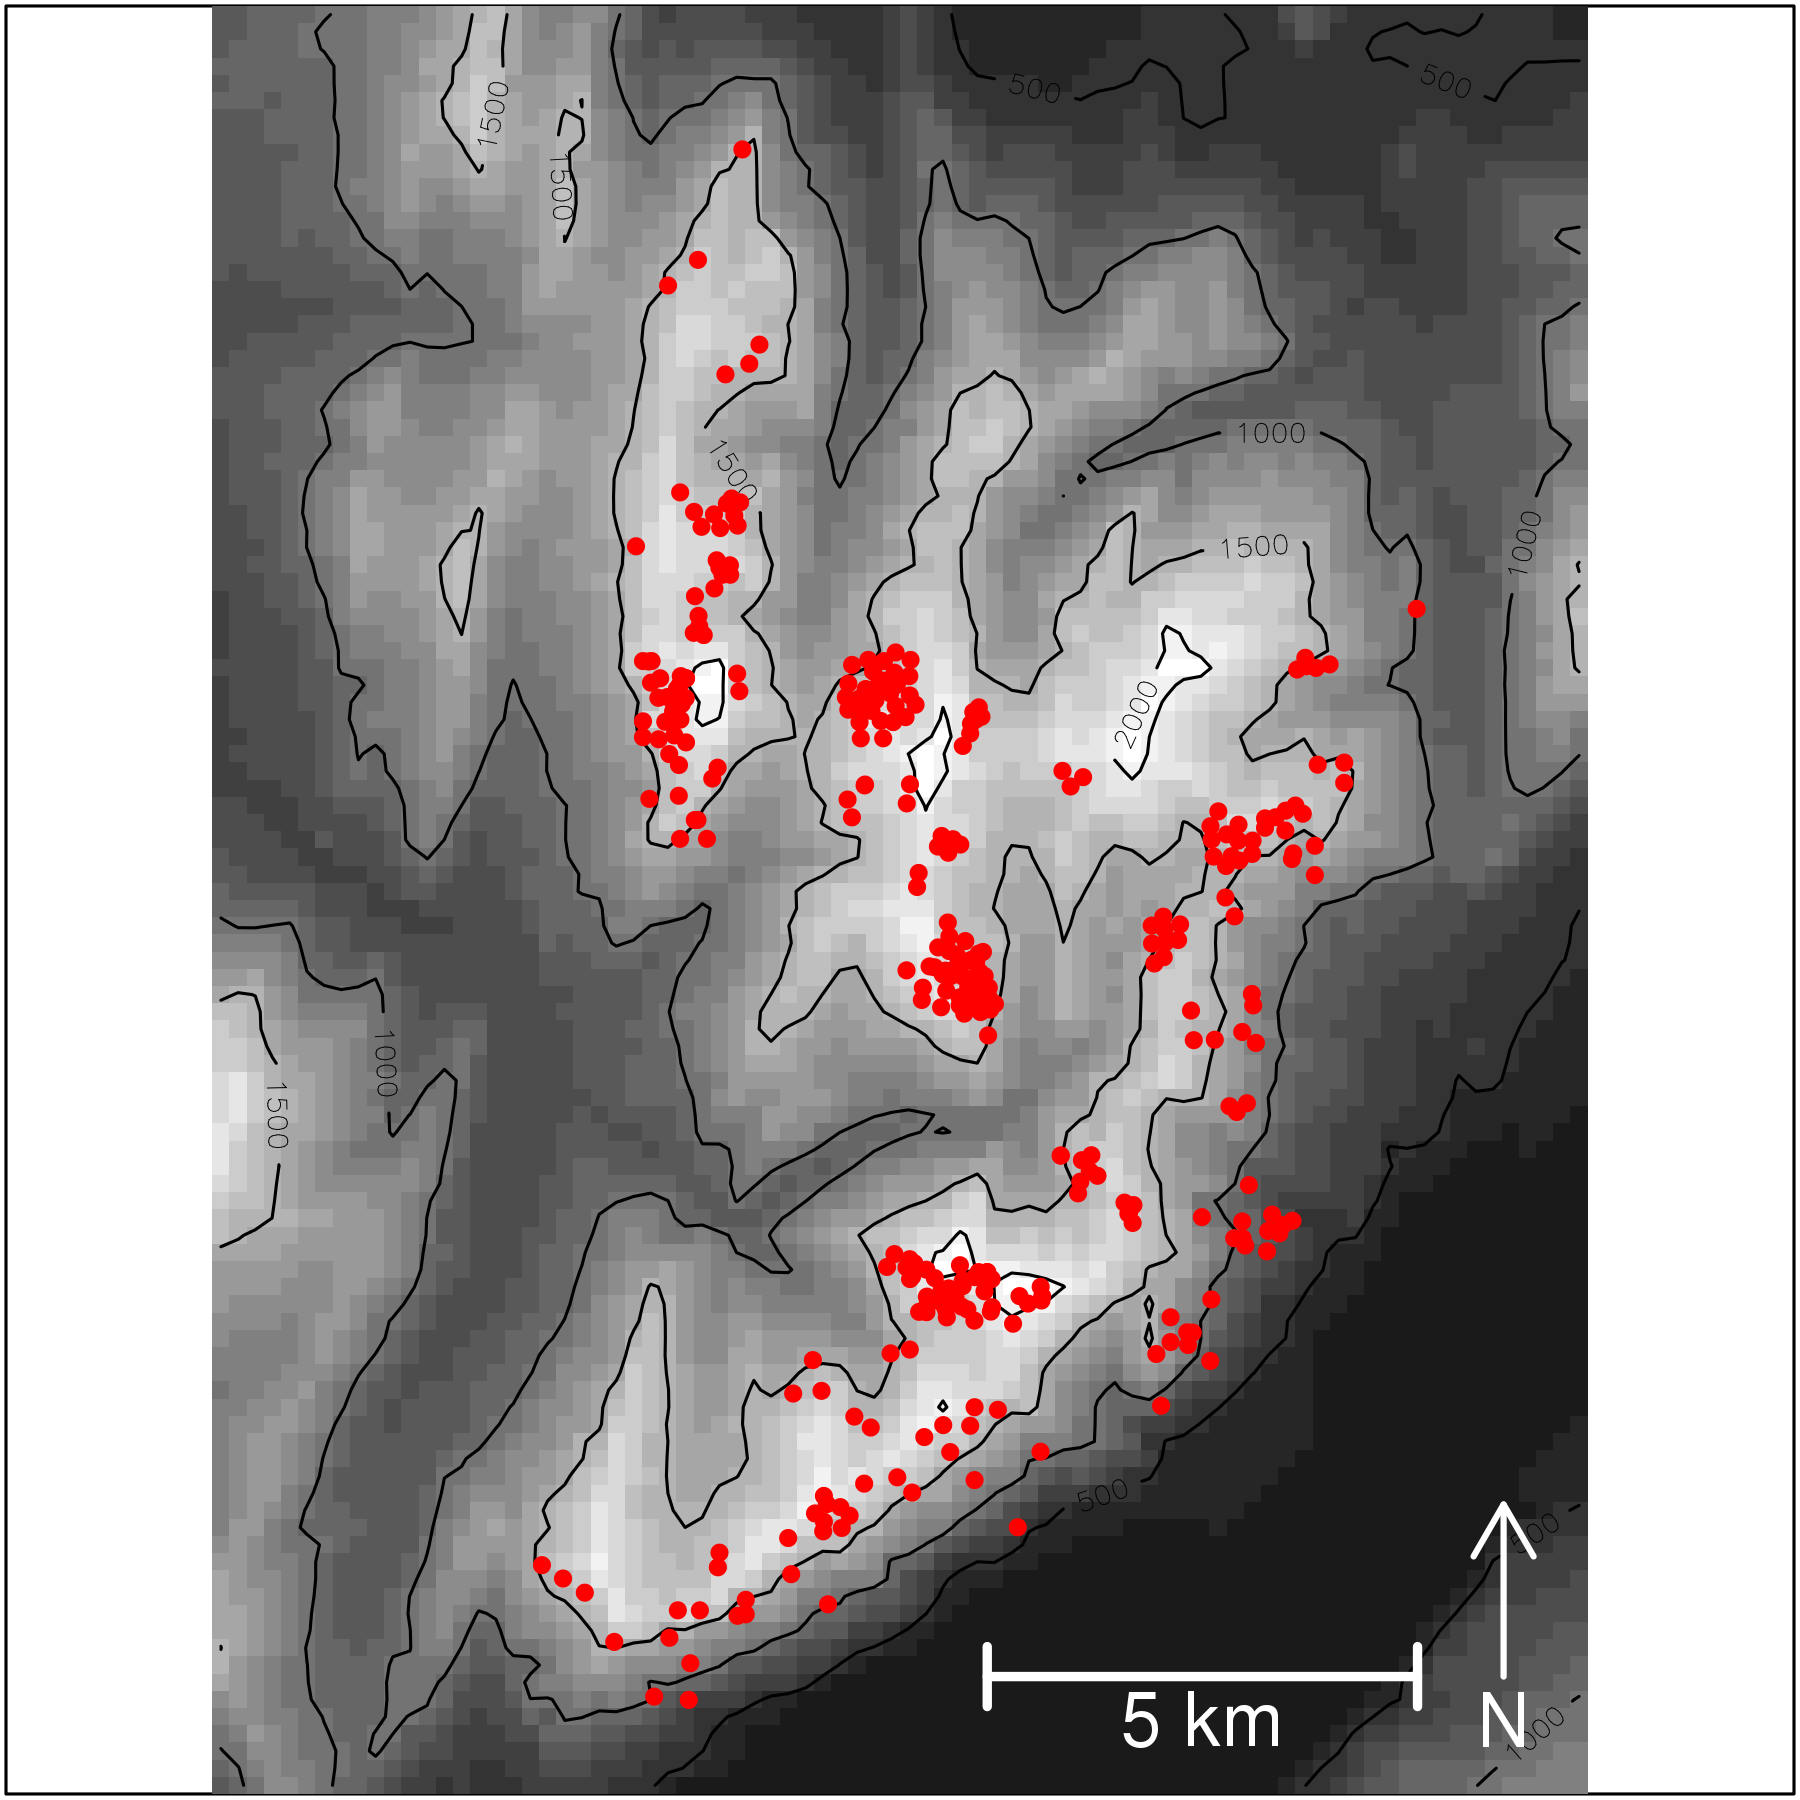
\includegraphics{figs/spca-023}

\noindent Alternatively, \texttt{filled.contour} can be used for the display, and a customized color
palette can be specified:
\begin{Schunk}
\begin{Sinput}
> myPal <- colorRampPalette(c("firebrick2", "white", "lightslateblue"))
> annot <- function() {
+     title("sPCA - interpolated map of individual scores")
+     points(x, y)
+ }
> filled.contour(temp, color.pal = myPal, nlev = 50, key.title = title("lagged \nscore 1"), 
+     plot.title = annot())
\end{Sinput}
\end{Schunk}
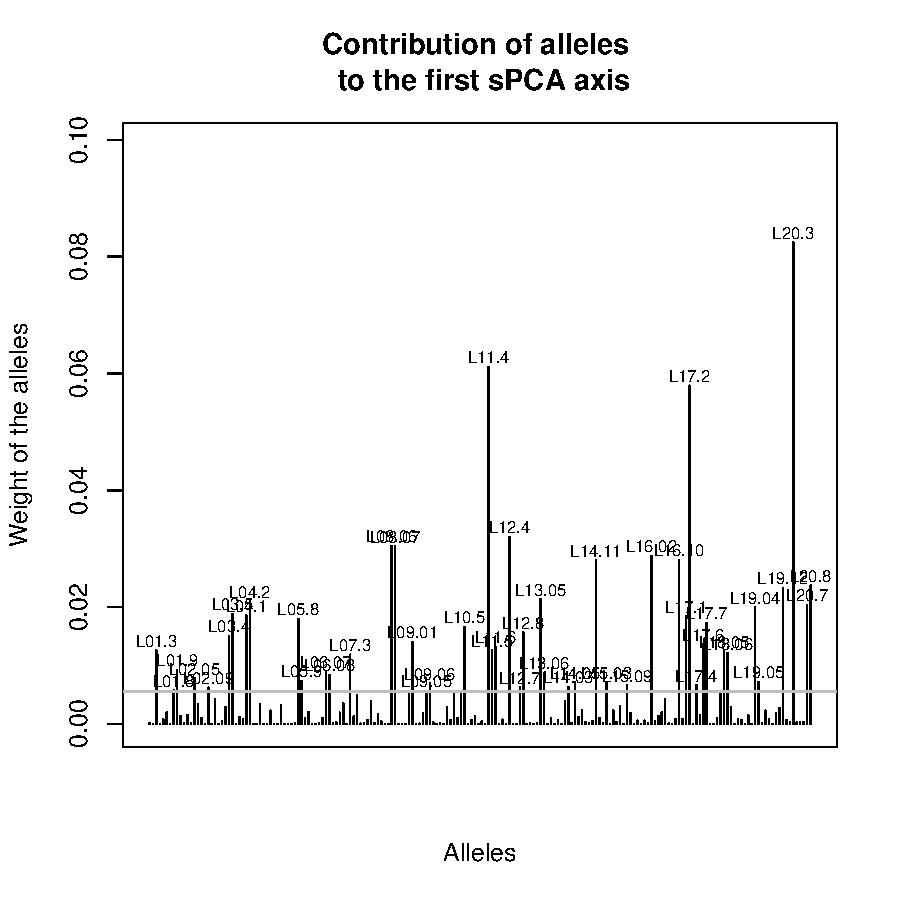
\includegraphics{figs/spca-024}
~\\


Besides assessing spatial patterns, it is sometimes valuable to assess which alleles actually
exhibit the structure of interest.
In sPCA, the contribution of alleles to a specific structure is given by the corresponding squared loading.
We can look for the alleles contributing most to e.g. the first axis
of sPCA, using the function \texttt{loadingplot} (see \texttt{?loadingplot} for
a description of the arguments):
\begin{Schunk}
\begin{Sinput}
> myLoadings <- mySpca$c1[, 1]^2
> names(myLoadings) <- rownames(mySpca$c1)
> loadingplot(myLoadings, xlab = "Alleles", ylab = "Weight of the alleles", 
+     main = "Contribution of alleles \n to the first sPCA axis")
\end{Sinput}
\end{Schunk}
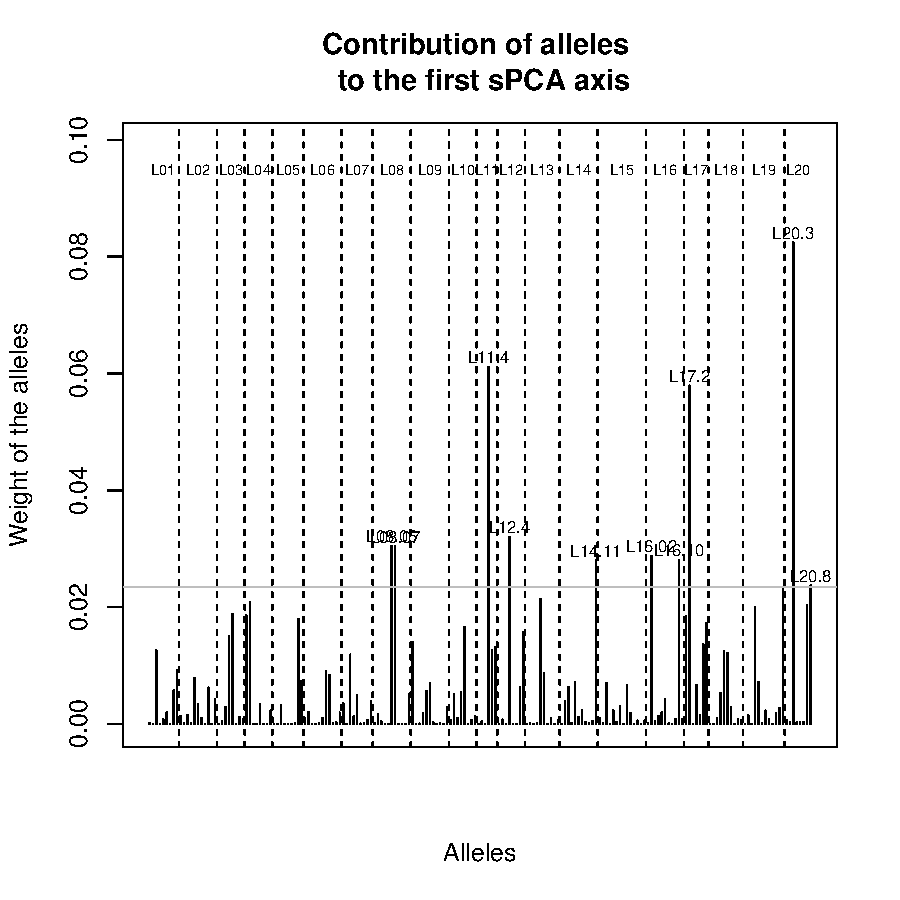
\includegraphics{figs/spca-025}

\noindent See \texttt{?loadingplot} for more information about this
function, in particular for the definition of the threshold value
above which alleles are annotated.
Note that it is possible to also separate the alleles by markers,
using the \texttt{fac} argument, to assess if all markers have
comparable contributions to a given structure.
In our case, we would only have to specify \texttt{fac=obj@loc.fac};
also note that \texttt{loadingplot} invisibly returns information
about the alleles whose contribution is above the threshold.
For instance, to identify the 5\% of alleles with the greatest
contributions to the first global structure in \texttt{mySpca}, we need:
\begin{Schunk}
\begin{Sinput}
> temp <- loadingplot(myLoadings, threshold = quantile(myLoadings, 
+     0.95), xlab = "Alleles", ylab = "Weight of the alleles", 
+     main = "Contribution of alleles \n to the first sPCA axis", 
+     fac = obj$loc.fac, cex.fac = 0.6)
> temp
\end{Sinput}
\begin{Soutput}
$threshold
       95% 
0.02345973 

$var.names
 [1] "L08.06" "L08.07" "L11.4"  "L12.4"  "L14.11" "L16.02" "L16.10" "L17.2" 
 [9] "L20.3"  "L20.8" 

$var.idx
L08.06 L08.07  L11.4  L12.4 L14.11 L16.02 L16.10  L17.2  L20.3  L20.8 
    71     72     99    105    130    146    154    157    187    192 

$var.values
    L08.06     L08.07      L11.4      L12.4     L14.11     L16.02     L16.10 
0.03044687 0.03037709 0.06111338 0.03199067 0.02799529 0.02873923 0.02806079 
     L17.2      L20.3      L20.8 
0.05793290 0.08246000 0.02368209 
\end{Soutput}
\end{Schunk}
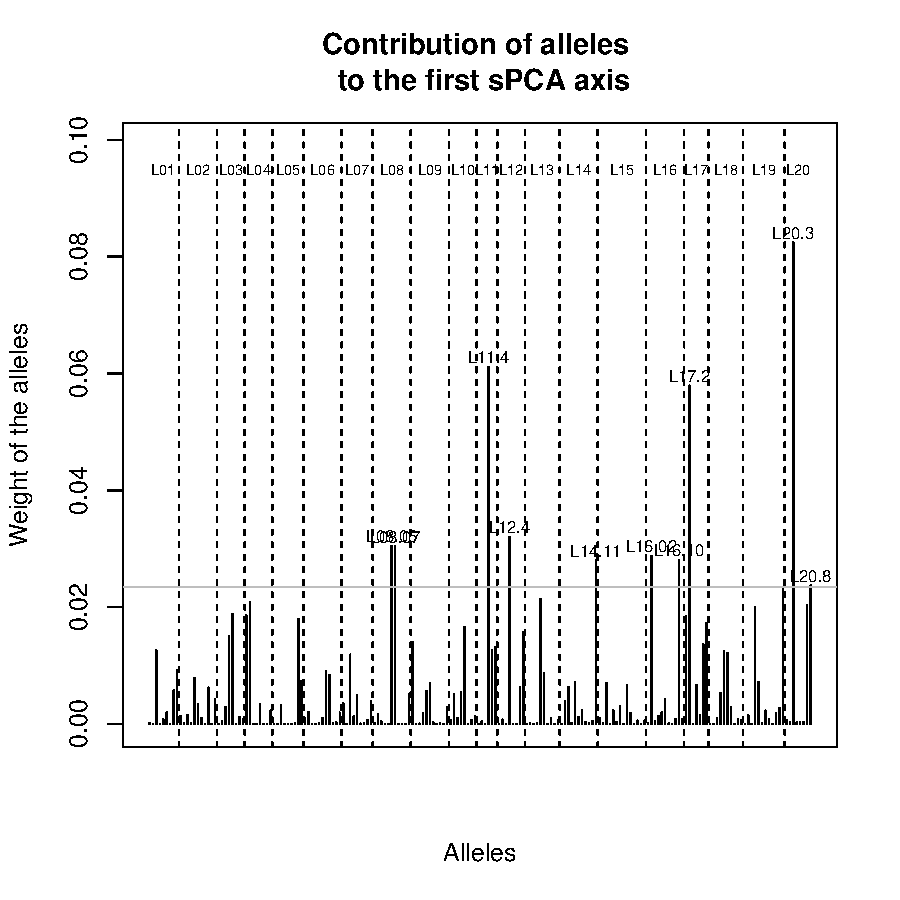
\includegraphics{figs/spca-026}

But to assess the average contribution of each marker, the
boxplot probably is a better tool:
\begin{Schunk}
\begin{Sinput}
> boxplot(myLoadings ~ obj$loc.fac, las = 3, ylab = "Contribution", 
+     xlab = "Marker", main = "Contributions by markers \nto the first global score", 
+     col = "grey")
\end{Sinput}
\end{Schunk}
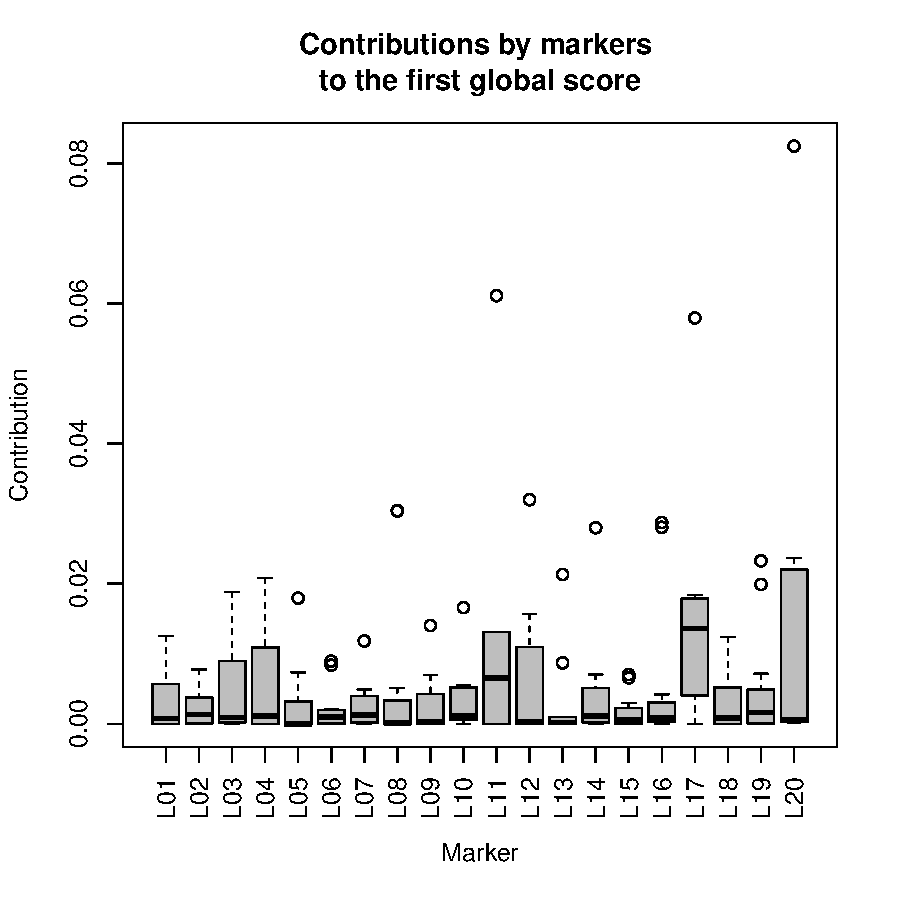
\includegraphics{figs/spca-boxplot}











%%%%%%%%%%%%%%%%%%%%%%%%%%
%%%%%%%%%%%%%%%%%%%%%%%%%%
\section{Case study: spatial genetic structure of the chamois in the Bauges mountains}
%%%%%%%%%%%%%%%%%%%%%%%%%%
%%%%%%%%%%%%%%%%%%%%%%%%%%
The chamois (\textit{Rupicapra rupicapra}) is a conserved species in France.
The Bauges mountains is a protected area in which the species has been
recently studied.
One of the most important questions for conservation purposes relates to whether individuals
from this area form a single reproductive unit, or whether they
are structured into sub-groups, and if so, what causes are likely to
induce this structuring.

While field observations are very scarce and do not allow to answer
this question, genetic data can be used to tackle the issue, as
departure from panmixia should result in genetic structuring.
The dataset \textit{rupica} contains 335 georeferenced genotypes of Chamois from the
Bauges mountains for 9 microsatellite markers, which we propose to
analyse.



%%%%%%%%%%%%%%%%%%%%%%%%%%
\subsection{An overview of the data}
%%%%%%%%%%%%%%%%%%%%%%%%%%
We first load the data:
\begin{Schunk}
\begin{Sinput}
> data(rupica)
> rupica
\end{Sinput}
\begin{Soutput}
   #####################
   ### Genind object ### 
   #####################
- genotypes of individuals - 

S4 class:  genind
@call: NULL

@tab:  335 x 55 matrix of genotypes

@ind.names: vector of  335 individual names
@loc.names: vector of  9 locus names
@loc.nall: number of alleles per locus
@loc.fac: locus factor for the  55 columns of @tab
@all.names: list of  9 components yielding allele names for each locus
@ploidy:  2
@type:  codom

Optionnal contents: 
@pop:  - empty -
@pop.names:  - empty -

@other: a list containing: xy  mnt  showBauges 
\end{Soutput}
\end{Schunk}
\texttt{rupica} is a \texttt{genind} object, that is, the class
of objects storing genotypes (as opposed to population data) in \textit{adegenet}.
\texttt{rupica} also contains topographic information about the
sampled area, which can be displayed by calling
\texttt{rupica\$other\$showBauges}.
Altitude maps are displayed using the \textit{adehabitat} package \cite{tj440}.
The spatial distribution of the sampling can be displayed as follows:
\begin{Schunk}
\begin{Sinput}
> rupica$other$showBauges()
> points(rupica$other$xy, col = "red", pch = 20)
\end{Sinput}
\end{Schunk}
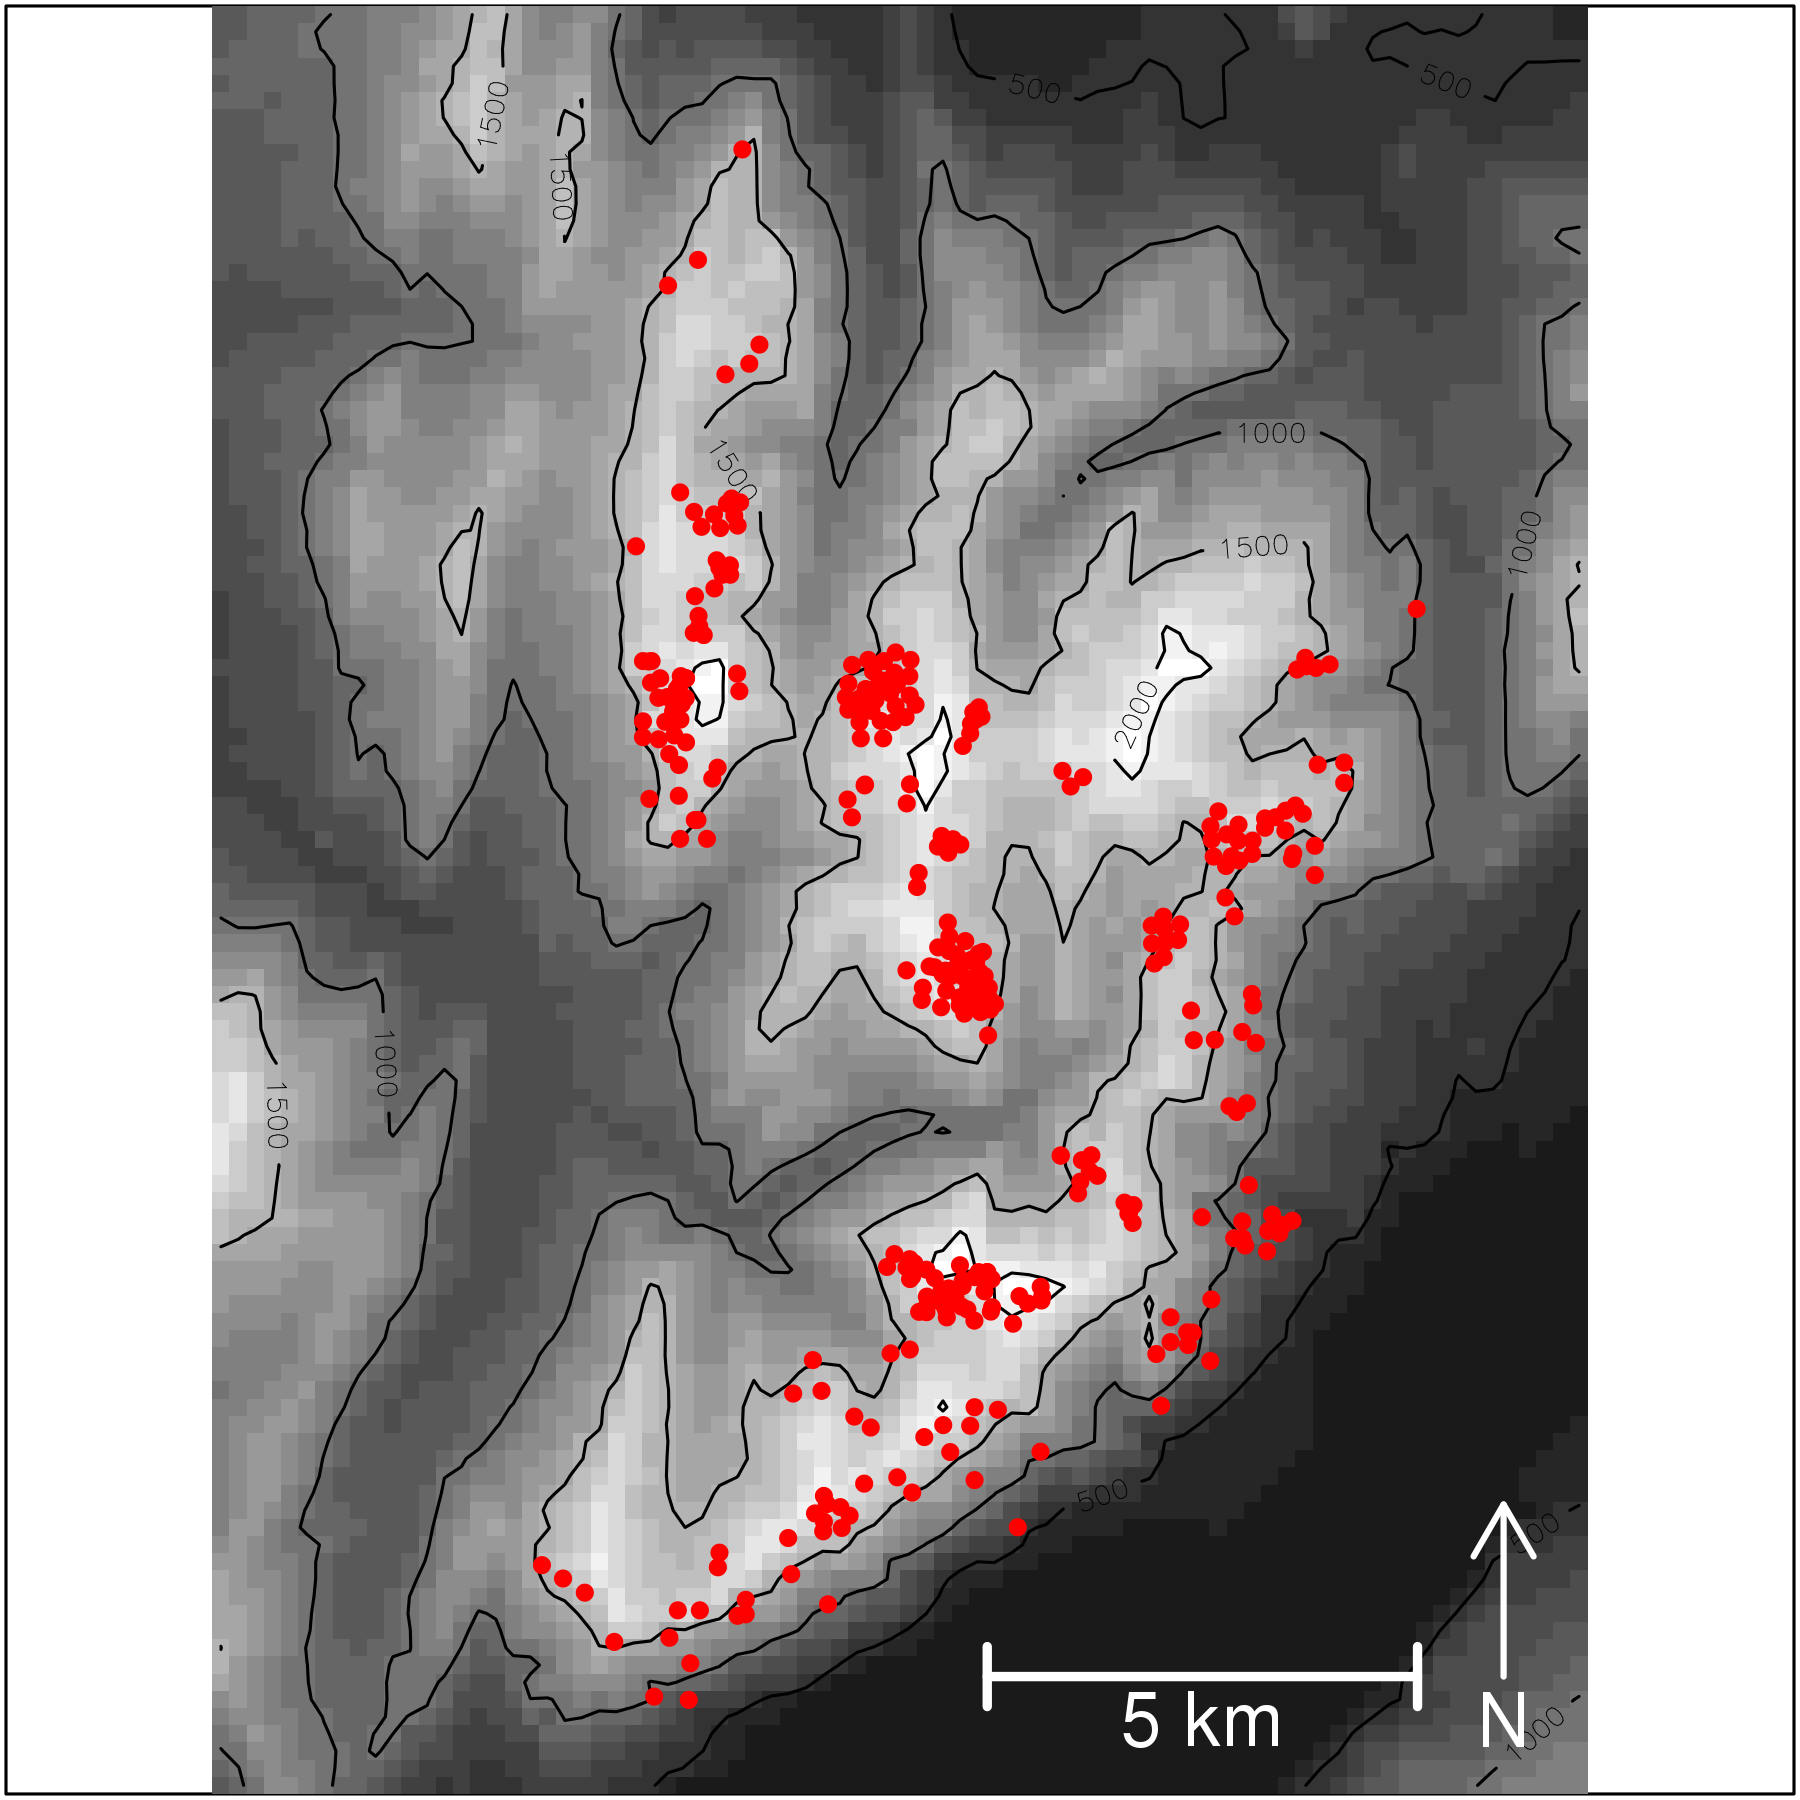
\includegraphics{figs/spca-029}

\noindent This spatial distribution is clearly not random, but seems arranged into
loose clusters.
However, superimposed samples can bias our visual assessment of the spatial clustering.
Use a two-dimensional kernel density estimation (function \texttt{s.kde2d}) to overcome this possible
issue.
\begin{Schunk}
\begin{Sinput}
> rupica$other$showBauges()
> s.kde2d(rupica$other$xy, add.plot = TRUE)
> points(rupica$other$xy, col = "red", pch = 20)
\end{Sinput}
\end{Schunk}
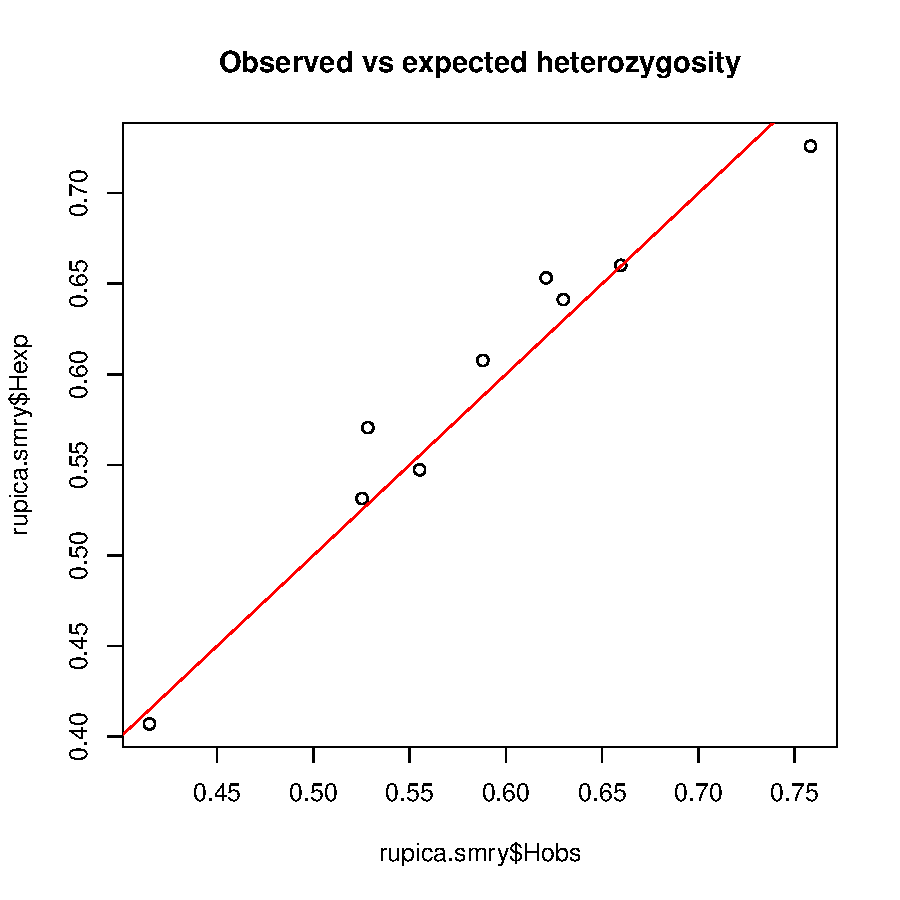
\includegraphics{figs/spca-030}

Unfortunately, geographical clustering is not strong enough to assign unambiguously each individual to a group.
Therefore, we need to carry all analyses at the individual level, which precludes the use of most
population genetics tools.




%%%%%%%%%%%%%%%%%%%%%%%%%%
\subsection{Summarising the genetic diversity}
%%%%%%%%%%%%%%%%%%%%%%%%%%
As a prior clustering of genotypes is not known, we cannot employ usual
$F_{ST}$-based approaches to detect genetic structuring.
However, genetic structure could still result in a deficit of
heterozygosity.
Use the \texttt{summary} of \texttt{genind} objects to compare expected and
observed heterozygosity:
\begin{Schunk}
\begin{Sinput}
> rupica.smry <- summary(rupica)
\end{Sinput}
\begin{Soutput}
 # Total number of genotypes:  335 

 # Population sample sizes:  
    
335 

 # Number of alleles per locus:  
L1 L2 L3 L4 L5 L6 L7 L8 L9 
 7 10  7  6  5  5  6  4  5 

 # Number of alleles per population:  
 1 
55 

 # Percentage of missing data:  
[1] 0

 # Observed heterozygosity:  
       L1        L2        L3        L4        L5        L6        L7        L8 
0.5880597 0.6208955 0.5253731 0.7582090 0.6597015 0.5283582 0.6298507 0.5552239 
       L9 
0.4149254 

 # Expected heterozygosity:  
       L1        L2        L3        L4        L5        L6        L7        L8 
0.6076769 0.6532517 0.5314591 0.7259657 0.6601604 0.5706082 0.6412742 0.5473112 
       L9 
0.4070709 
\end{Soutput}
\begin{Sinput}
> plot(rupica.smry$Hobs, rupica.smry$Hexp, main = "Observed vs expected heterozygosity")
> abline(0, 1, col = "red")
\end{Sinput}
\end{Schunk}
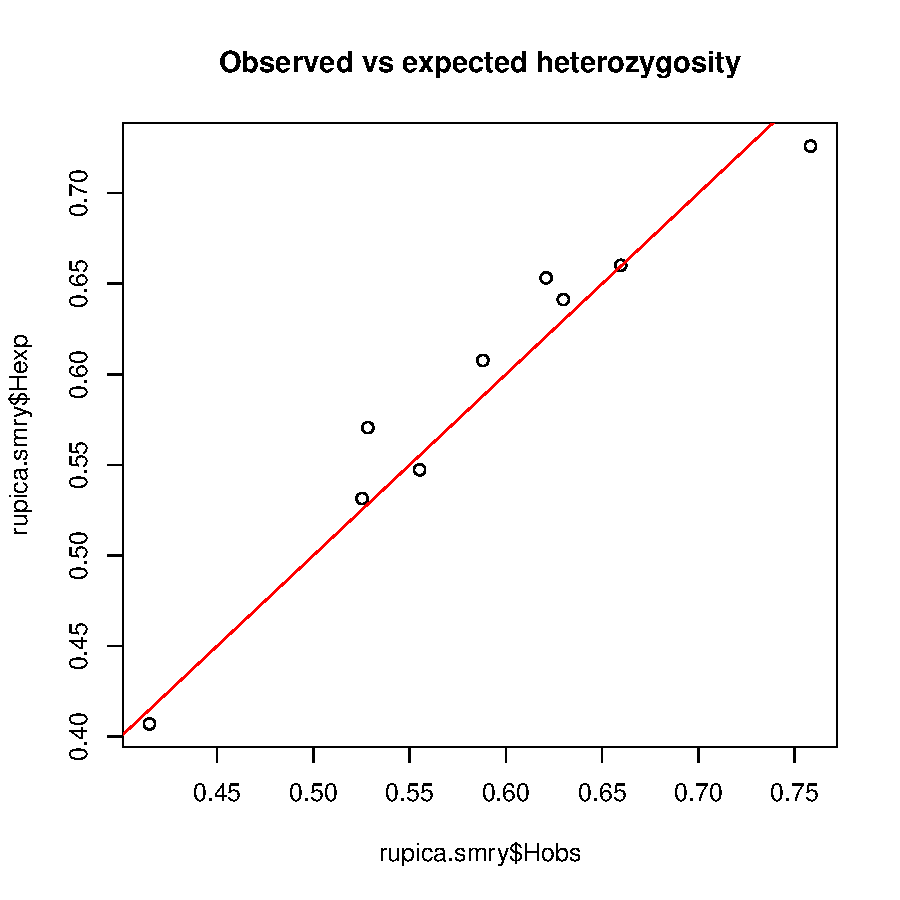
\includegraphics{figs/spca-031}

\noindent The red line indicate identity between both quantities.
Observed heterozygosity do not seem to deviate massively from theoretical expectations.
This is confirmed by a classical pairwise $t$-test::
\begin{Schunk}
\begin{Sinput}
> t.test(rupica.smry$Hexp, rupica.smry$Hobs, paired = TRUE, var.equal = TRUE)
\end{Sinput}
\begin{Soutput}
	Paired t-test

data:  rupica.smry$Hexp and rupica.smry$Hobs 
t = 0.9461, df = 8, p-value = 0.3718
alternative hypothesis: true difference in means is not equal to 0 
95 percent confidence interval:
 -0.01025068  0.02451318 
sample estimates:
mean of the differences 
            0.007131251 
\end{Soutput}
\end{Schunk}
~\\

We can seek a global picture of the genetic diversity among genotypes
using a Principal Component Analysis (PCA, function \texttt{dudi.pca} in the \texttt{ade4}
package).
The analysis is performed on a table of standardized alleles
frequencies, obtained by \texttt{scaleGen} (use the binomial scaling option).
Note that we disable the scaling option when performing the PCA, which would otherwise re-scale the
data and therefore erase the previous scaling of \texttt{scaleGen}.
The function \texttt{dudi.pca} displays a barplot of
eigenvalues and asks for a number of retained principal components:
\begin{Schunk}
\begin{Sinput}
> rupica.X <- scaleGen(rupica, method = "binom")
> rupica.pca1 <- dudi.pca(rupica.X, cent = FALSE, scale = FALSE, 
+     scannf = FALSE, nf = 2)
> barplot(rupica.pca1$eig, main = "Rupica dataset - PCA eigenvalues", 
+     col = heat.colors(length(rupica.pca1$eig)))
\end{Sinput}
\end{Schunk}
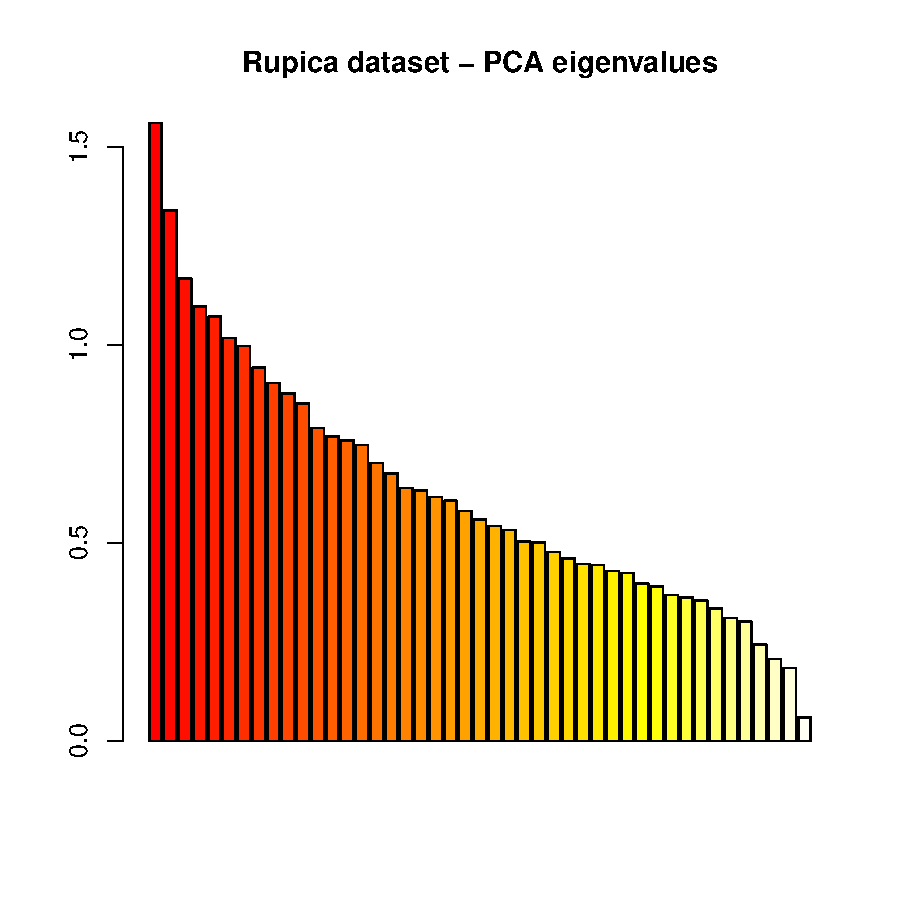
\includegraphics{figs/spca-033}

\noindent The output produced by \texttt{dudi.pca} is a \texttt{dudi} object.
A \texttt{dudi} object contains various information; in the case of
PCA, principal axes (loadings), principal components (synthetic variable), and eigenvalues are respectively
stored in \texttt{\$c1}, \texttt{\$li}, and \texttt{\$eig} slots.
Here is the content of the PCA:
\begin{Schunk}
\begin{Sinput}
> rupica.pca1
\end{Sinput}
\begin{Soutput}
Duality diagramm
class: pca dudi
$call: dudi.pca(df = rupica.X, center = FALSE, scale = FALSE, scannf = FALSE, 
    nf = 2)

$nf: 2 axis-components saved
$rank: 45
eigen values: 1.561 1.34 1.168 1.097 1.071 ...
  vector length mode    content       
1 $cw    55     numeric column weights
2 $lw    335    numeric row weights   
3 $eig   45     numeric eigen values  

  data.frame nrow ncol content             
1 $tab       335  55   modified array      
2 $li        335  2    row coordinates     
3 $l1        335  2    row normed scores   
4 $co        55   2    column coordinates  
5 $c1        55   2    column normed scores
other elements: cent norm 
\end{Soutput}
\end{Schunk}

In general, eigenvalues represent the amount of genetic diversity --- as measured by
the multivariate method being used --- represented by each principal component (PC).
An abrupt decrease in eigenvalues is likely to indicate the boundary
between true patterns and non-interpretable structures.
In this case, the first two PCs may contain some relevant biological signal.
\\


We can use \texttt{s.label} to display the two first components of the analysis.
Kernel density estimation (\texttt{s.kde2d}) is used for a better
assessment of the distribution of the genotypes onto the principal axes:
\begin{Schunk}
\begin{Sinput}
> s.label(rupica.pca1$li)
> s.kde2d(rupica.pca1$li, add.p = TRUE, cpoint = 0)
> add.scatter.eig(rupica.pca1$eig, 2, 1, 2)
\end{Sinput}
\end{Schunk}
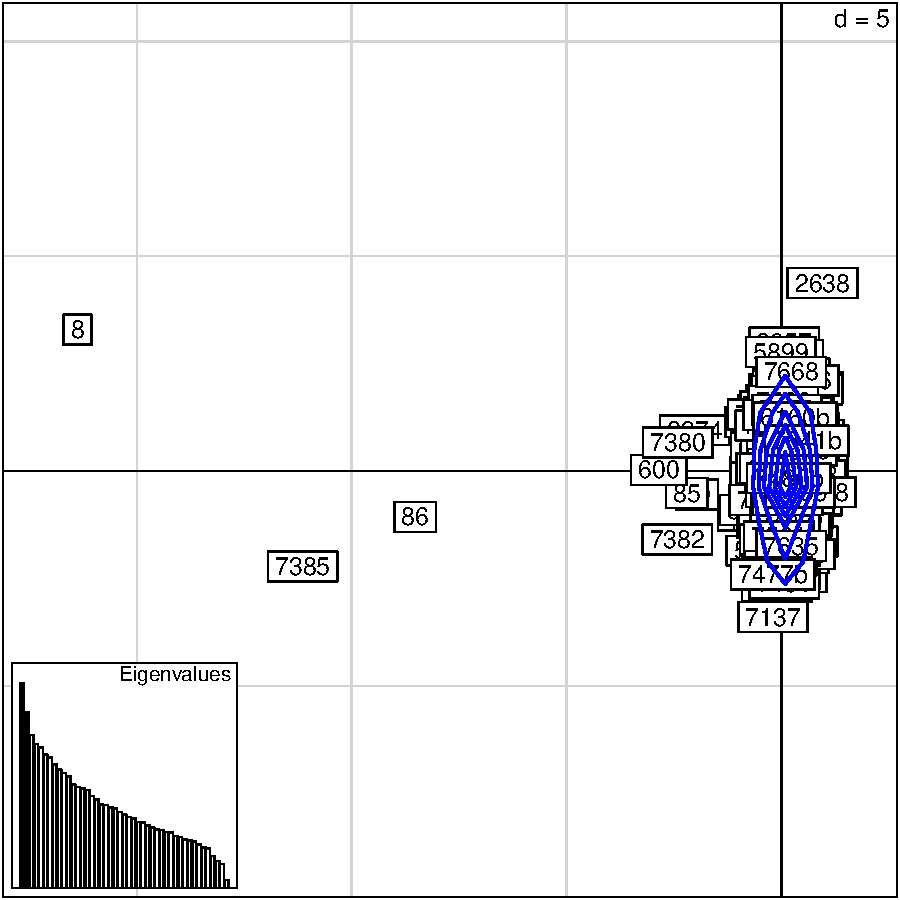
\includegraphics{figs/spca-035}

\noindent This scatterplot shows that the only structure identified by PCA points to a few outliers.
\texttt{loadingplot} confirms that this corresponds to the possession of a few original alleles:
\begin{Schunk}
\begin{Sinput}
> loadingplot(rupica.pca1$c1^2)
\end{Sinput}
\end{Schunk}
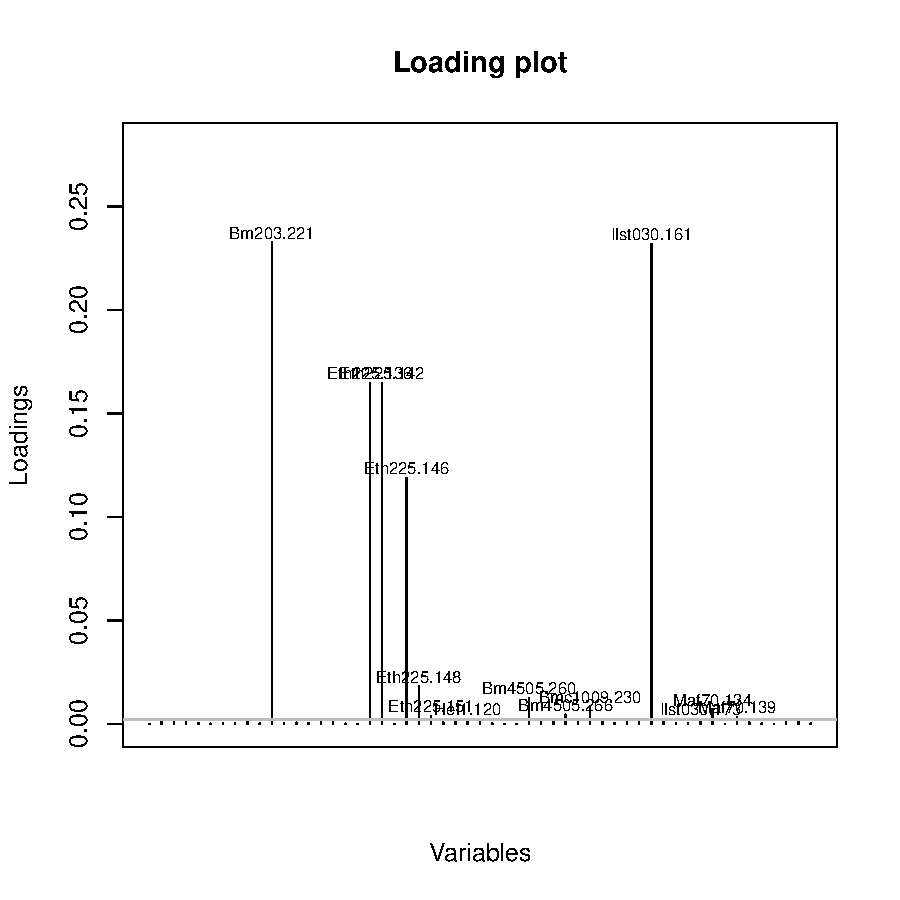
\includegraphics{figs/spca-036}

\noindent We can go back to the genotypes for the concerned markers (e.g.,
Bm203) to check whether the highlighted genotypes are uncommon.
\texttt{truenames} extracts the table of allele frequencies from a
\texttt{genind} object (restoring original labels for markers, alleles, and individuals):
\begin{Schunk}
\begin{Sinput}
> X <- truenames(rupica)
> class(X)
\end{Sinput}
\begin{Soutput}
[1] "matrix"
\end{Soutput}
\begin{Sinput}
> dim(X)
\end{Sinput}
\begin{Soutput}
[1] 335  55
\end{Soutput}
\begin{Sinput}
> bm203.221 <- X[, "Bm203.221"]
> table(bm203.221)
\end{Sinput}
\begin{Soutput}
bm203.221
                  0 0.00597014925373134                 0.5 
                330                   1                   4 
\end{Soutput}
\end{Schunk}
Only 4 genotypes possess one copy of the allele 221 of marker bm203 (the second result
corresponds to a replaced missing data).
Which individuals are they?
\begin{Schunk}
\begin{Sinput}
> rownames(X)[bm203.221 == 0.5]
\end{Sinput}
\begin{Soutput}
   001    019    029    276 
   "8"   "86"  "600" "7385" 
\end{Soutput}
\end{Schunk}
These are indeed our outliers.
From the point of view of PCA, this would be the only structure in the data.
However, further analyses show that more is to be seen...
\\






%%%%%%%%%%%%%%%%%%%%%%%%%%
\subsection{Mapping and testing PCA results}
%%%%%%%%%%%%%%%%%%%%%%%%%%
A frequent practice in spatial genetics is mapping the first principal components (PCs) onto the geographic space.
\textit{ade4}'s function \texttt{s.value} is well-suited to do so, using black and
white squares of variable size for positive and negative values.
To give a legend for this type of representation:
\begin{Schunk}
\begin{Sinput}
> s.value(cbind(1:11, rep(1, 11)), -5:5, cleg = 0)
> text(1:11, rep(1, 11), -5:5, col = "red", cex = 1.5)
\end{Sinput}
\end{Schunk}
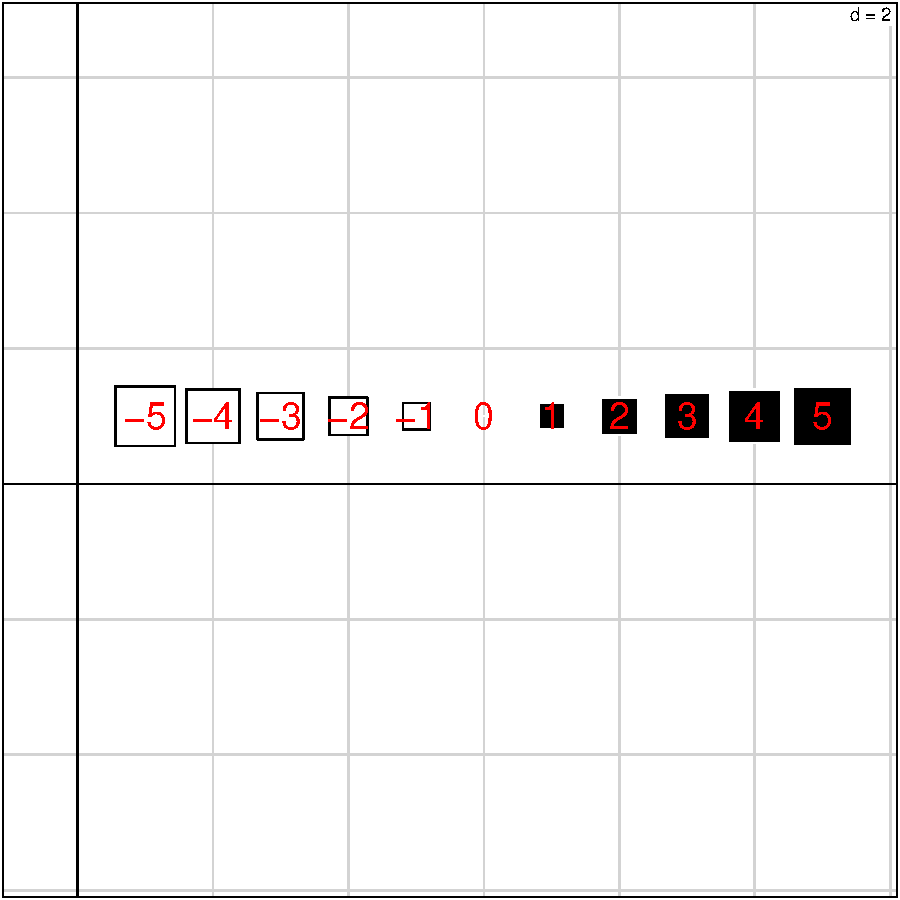
\includegraphics{figs/spca-svaluedem}

\noindent We apply this graphical representation to the first
two PCs of the PCA:
\begin{Schunk}
\begin{Sinput}
> showBauges <- rupica$other$showBauges
> showBauges()
> s.value(rupica$other$xy, rupica.pca1$li[, 1], add.p = TRUE, cleg = 0.5)
> title("PCA - first PC", col.main = "yellow", line = -2, cex.main = 2)
\end{Sinput}
\end{Schunk}
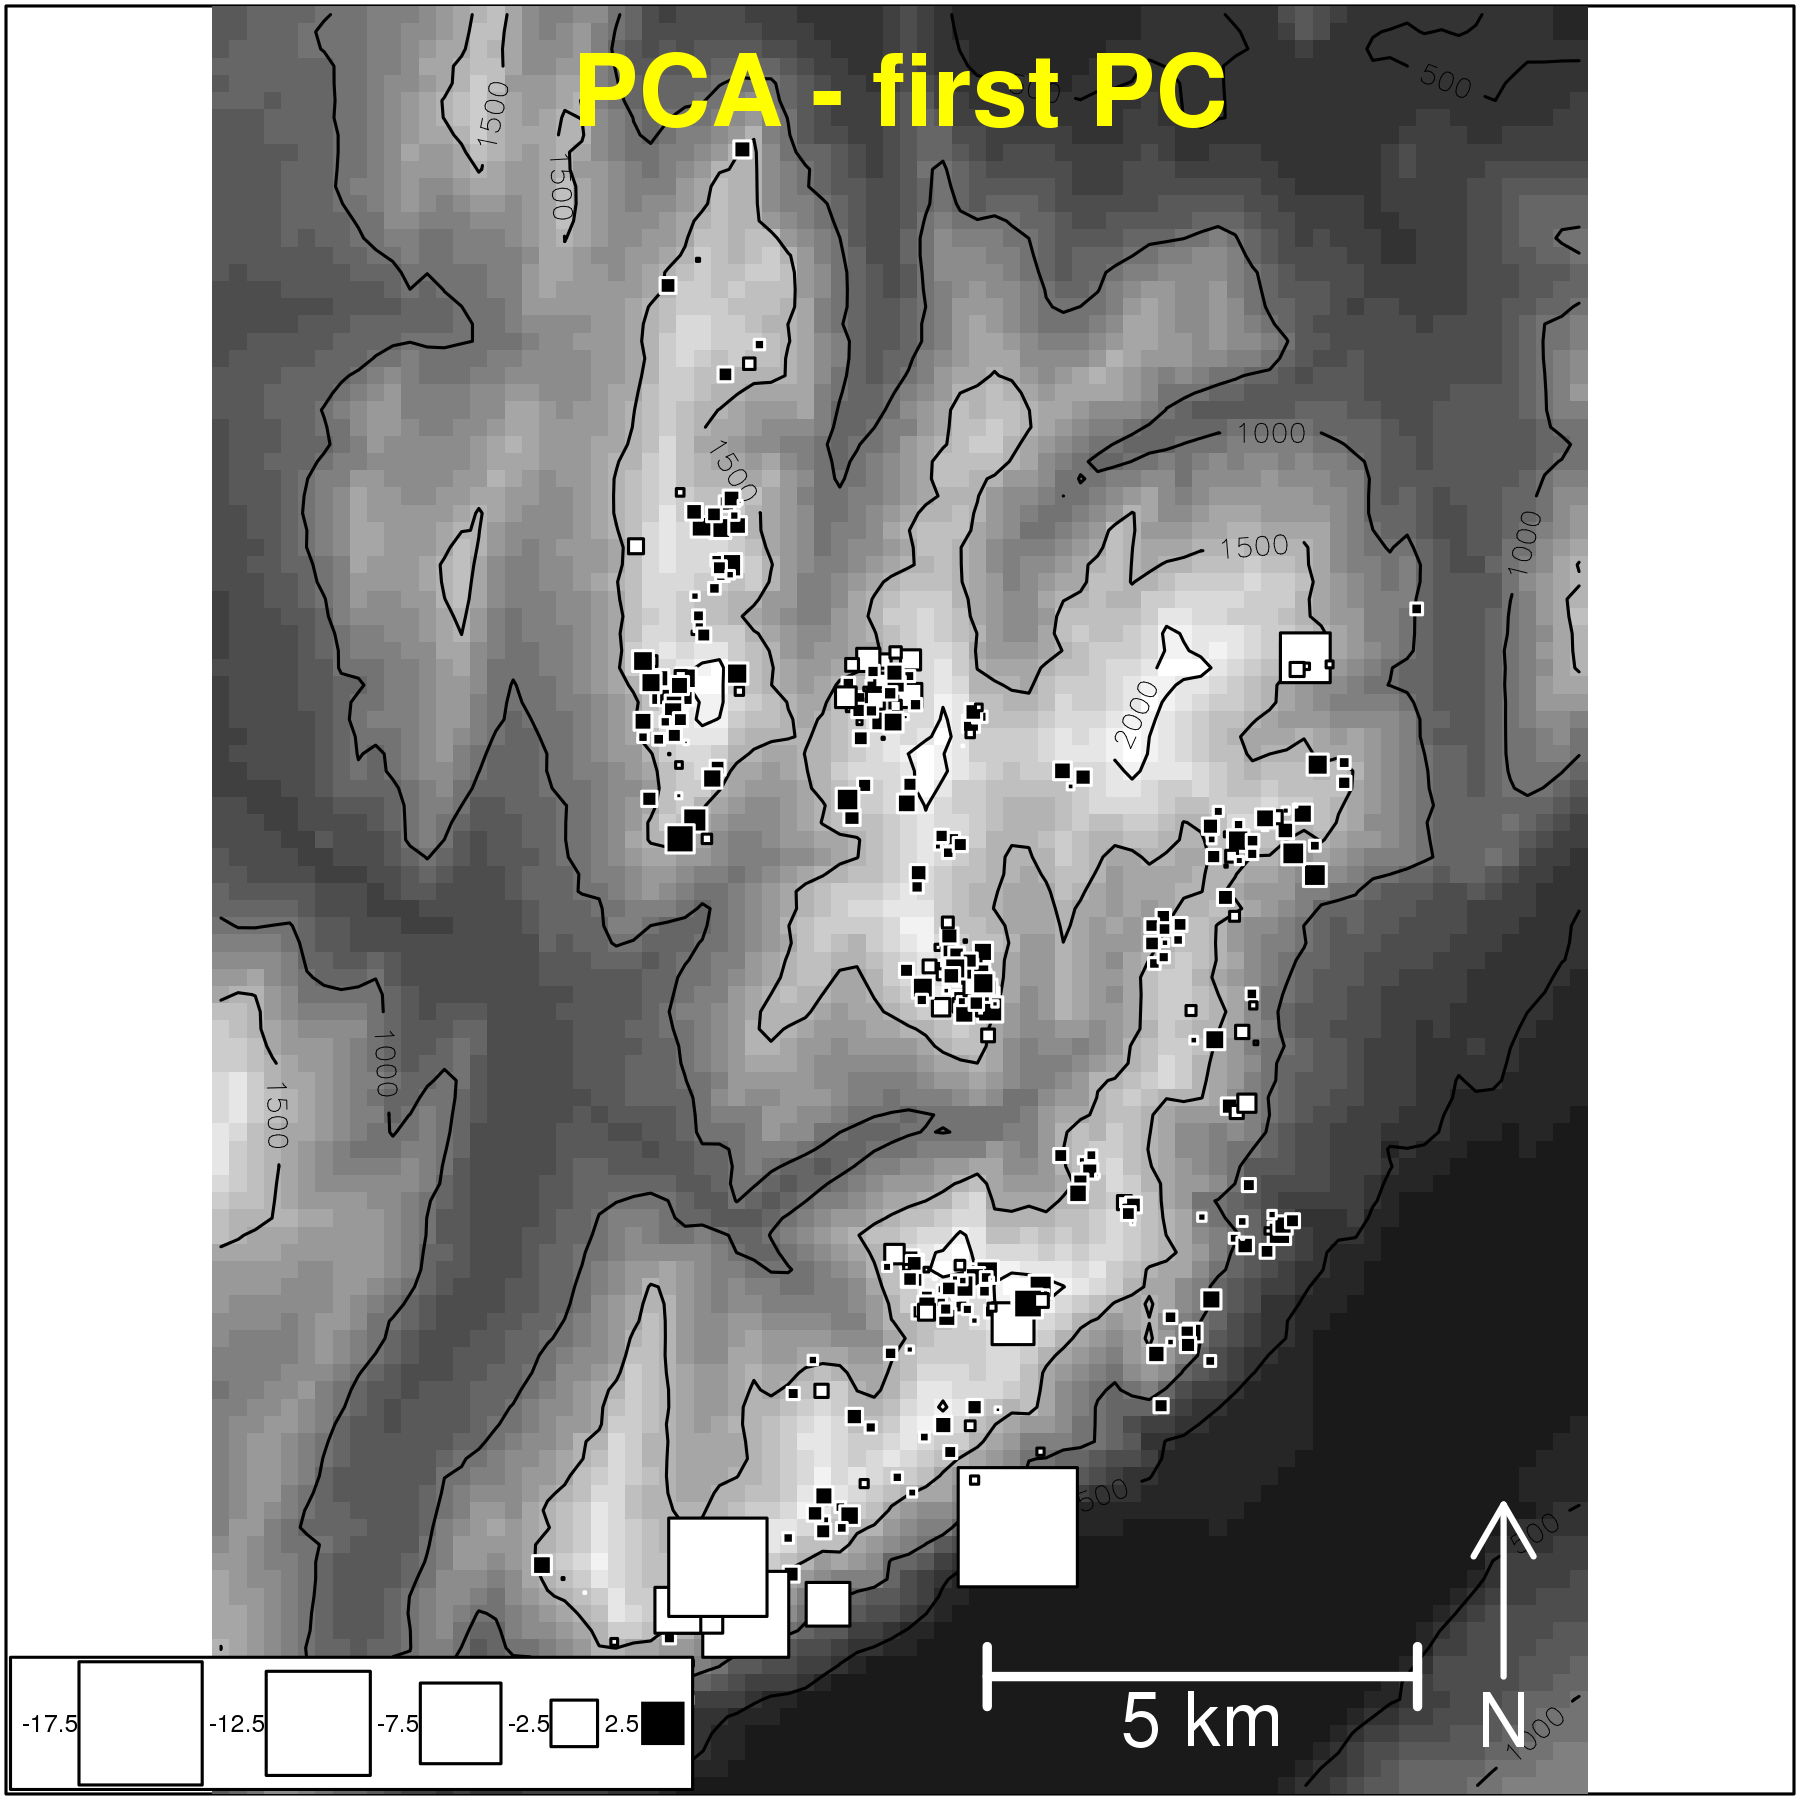
\includegraphics{figs/spca-040}

\begin{Schunk}
\begin{Sinput}
> showBauges()
> s.value(rupica$other$xy, rupica.pca1$li[, 2], add.p = TRUE, csize = 0.7)
> title("PCA - second PC", col.main = "yellow", line = -2, cex.main = 2)
\end{Sinput}
\end{Schunk}
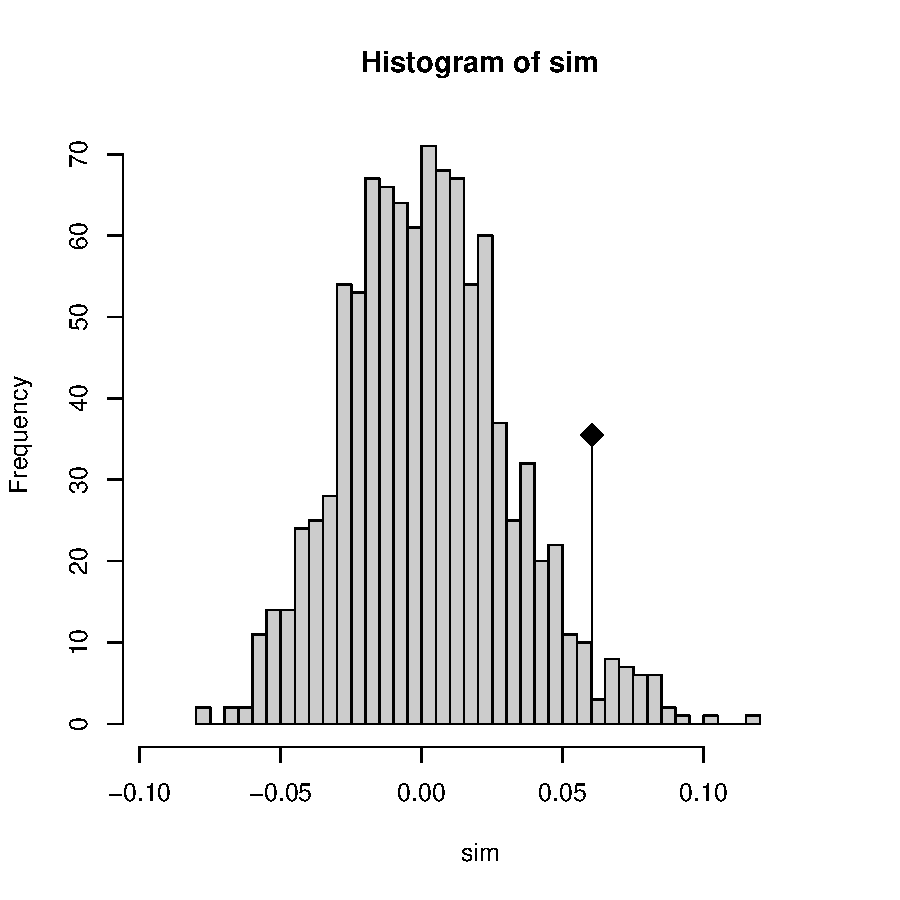
\includegraphics{figs/spca-041}


\noindent As we can see, none of these PCs seems to display a particular spatial pattern.
This visual assessment can be complemented by a test of spatial autocorrelation in these PCs.
This can be achieved using Moran's $I$ test.
We use \textit{spdep}'s function \texttt{moran.mc} to perform these two tests.
We first need to define the spatial connectivity between the sampled individuals.
For these data, spatial connectivity is best defined as the overlap between home ranges of
individuals, modelled as disks with a radius of 1150m.
\texttt{chooseCN} is used to create the corresponding connection network:
\begin{Schunk}
\begin{Sinput}
> rupica.graph <- chooseCN(rupica$other$xy, type = 5, d1 = 0, d2 = 2300, 
+     plot = FALSE, res = "listw")
\end{Sinput}
\end{Schunk}
The connection network should ressemble this:
\begin{Schunk}
\begin{Sinput}
> rupica.graph
\end{Sinput}
\begin{Soutput}
Characteristics of weights list object:
Neighbour list object:
Number of regions: 335 
Number of nonzero links: 18018 
Percentage nonzero weights: 16.05525 
Average number of links: 53.78507 

Weights style: W 
Weights constants summary:
    n     nn  S0       S1      S2
W 335 112225 335 15.04311 1352.07
\end{Soutput}
\begin{Sinput}
> plot(rupica.graph, rupica$other$xy)
> title("rupica.graph")
\end{Sinput}
\end{Schunk}
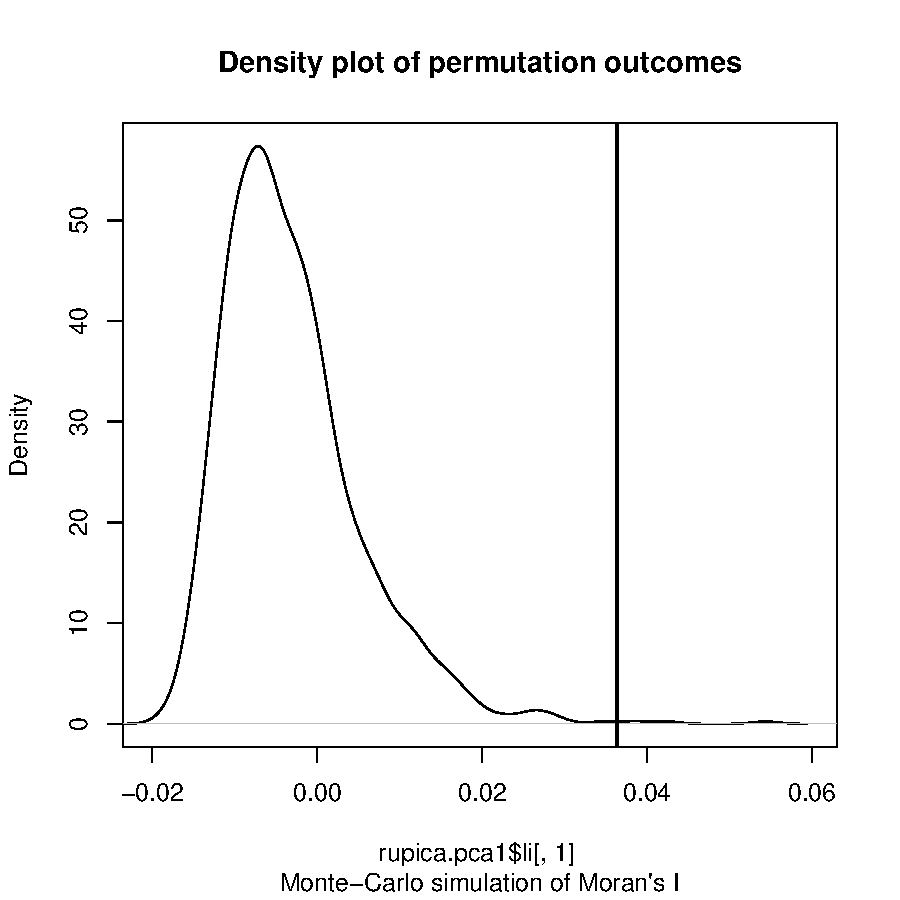
\includegraphics{figs/spca-043}

We perform Moran's test for the first two PCs, and plot the results.
\begin{Schunk}
\begin{Sinput}
> pc1.mctest <- moran.mc(rupica.pca1$li[, 1], rupica.graph, 999)
> plot(pc1.mctest)
\end{Sinput}
\end{Schunk}
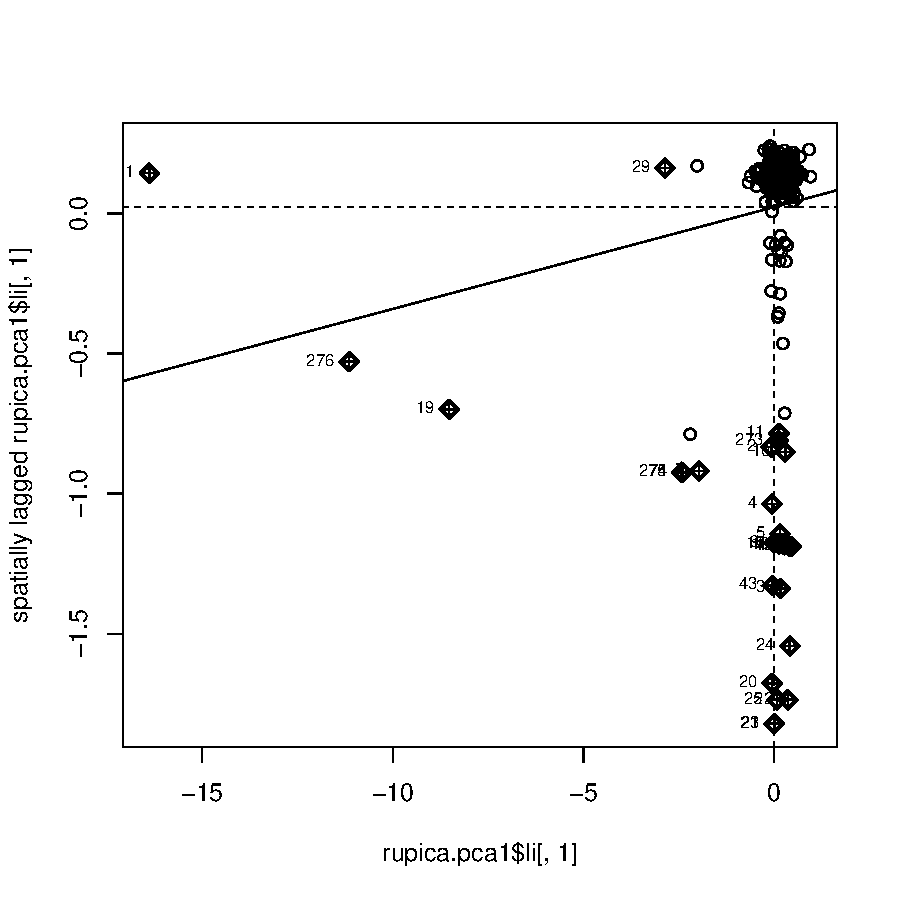
\includegraphics{figs/spca-044}

\noindent This result is surprisingly significant. Why is this?
Moran's plot (\texttt{moran.plot}) represents the tested variable against its lagged vector; we
apply it to the first PC:
\begin{Schunk}
\begin{Sinput}
> moran.plot(rupica.pca1$li[, 1], rupica.graph)
\end{Sinput}
\end{Schunk}
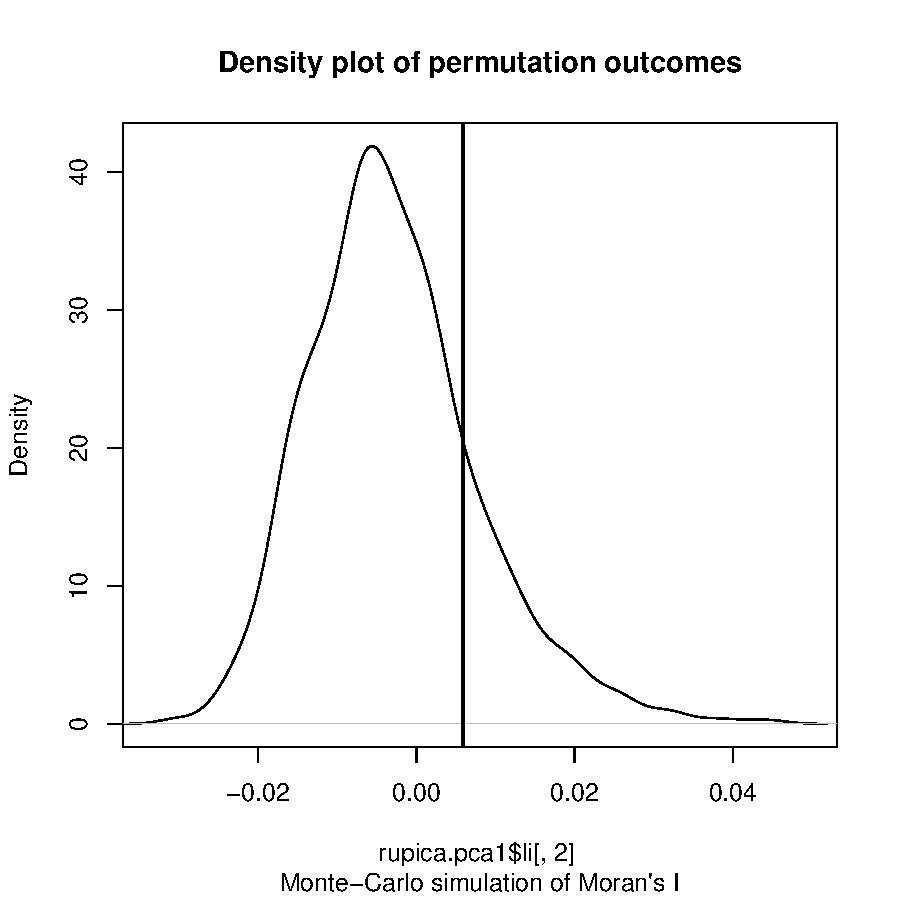
\includegraphics{figs/spca-045}

\noindent Positive autocorrelation corresponds to a positive correlation between a variable
and its lag vector.
Here, we can see that this relation is entirely driven by the previously identified outliers, which
turn out to be neighbours.
This is therefore a fairly trivial and uninteresting pattern.
Results obtained on the second PC are less surprisingly non-significant:
\begin{Schunk}
\begin{Sinput}
> pc2.mctest <- moran.mc(rupica.pca1$li[, 2], rupica.graph, 999)
> plot(pc2.mctest)
\end{Sinput}
\end{Schunk}
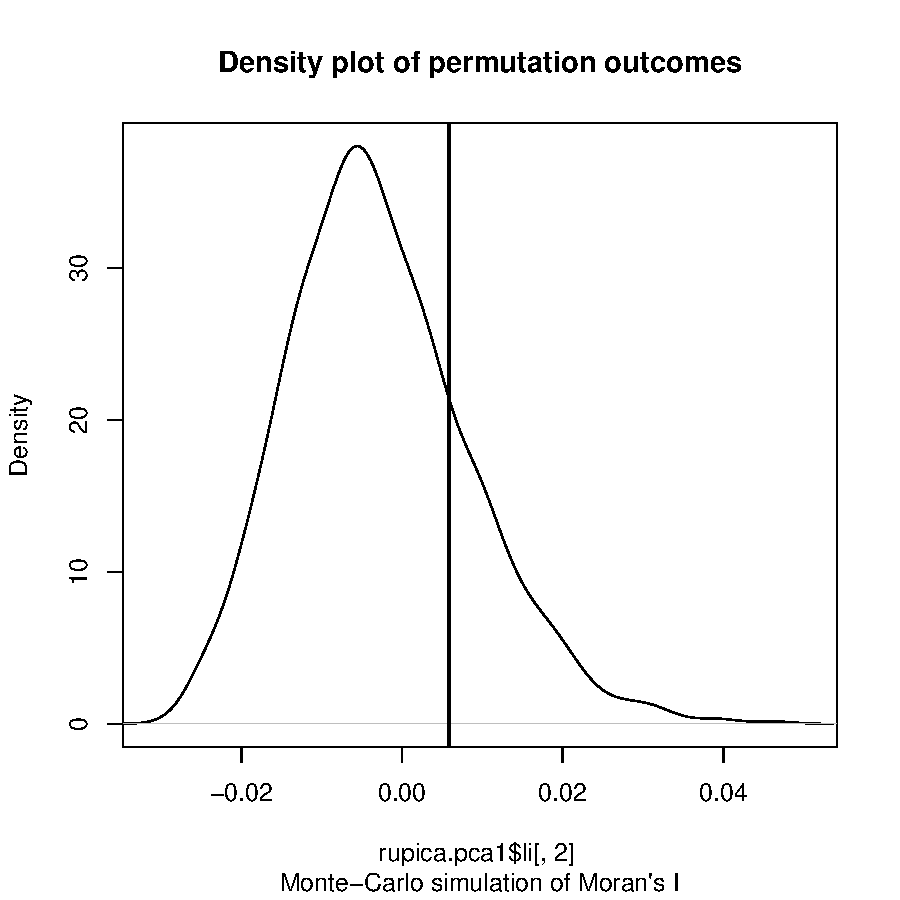
\includegraphics{figs/spca-046}







%%%%%%%%%%%%%%%%%%%%%%%%%%
\subsection{Multivariate tests of spatial structure}
%%%%%%%%%%%%%%%%%%%%%%%%%%
So far, we have only tested the existence of spatial structures in the first two principal components
of a PCA of the data.
Therefore, these tests only describe one fragment of the data, and do not encompass the whole
diversity in the data.
As a complement, we can use Mantel test (\texttt{mantel.randtest}) to test spatial structures in the
whole data, by assessing the correlation between genetic distances and geographic distances.
Pairwise Euclidean distances are computed using \texttt{dist}.
Perform Mantel test, using the scaled genetic data you used before in PCA, and the geographic coordinates.
\begin{Schunk}
\begin{Sinput}
> mtest <- mantel.randtest(dist(rupica.X), dist(rupica$other$xy))
> plot(mtest, nclass = 30)
\end{Sinput}
\end{Schunk}
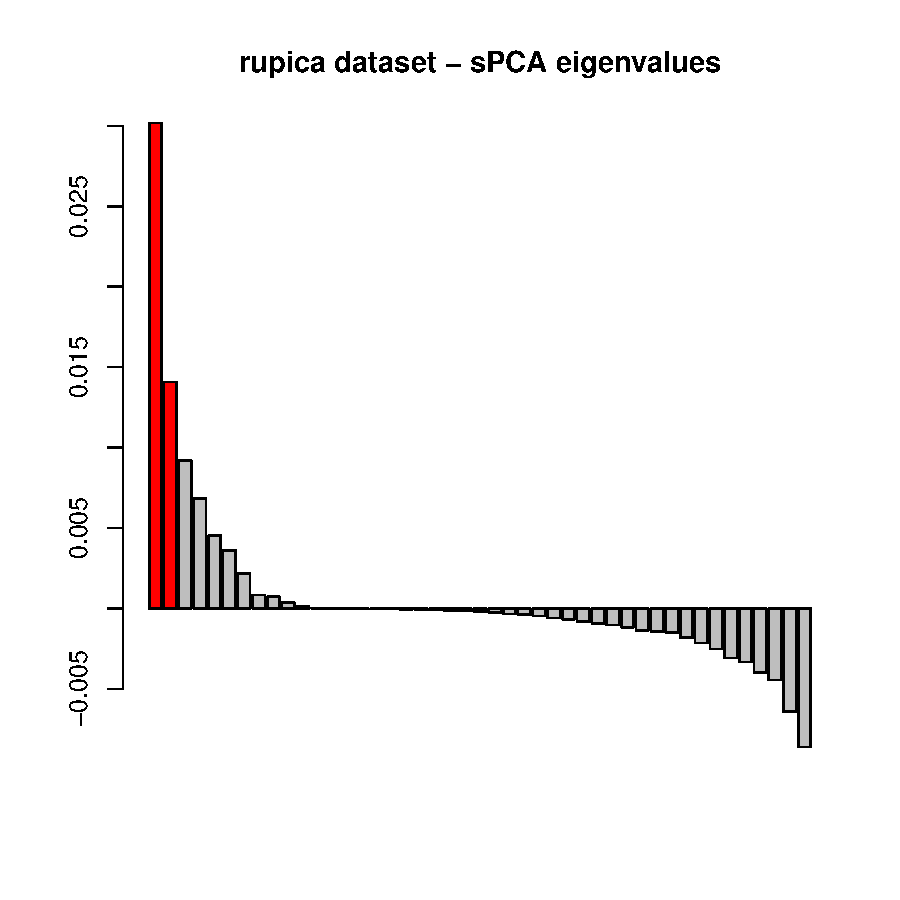
\includegraphics{figs/spca-047}

\noindent Interestingly, this test turns out to be marginally significant, and would encourage us to
look for spatial patterns. This is the role of the spatial Principal Component Analysis.





%%%%%%%%%%%%%%%%%%%%%%%%%%
\subsection{Spatial Principal Component Analysis}
%%%%%%%%%%%%%%%%%%%%%%%%%%

We apply an sPCA to the \texttt{rupica} dataset, using the connection network used previously in
Moran's $I$ tests:
\begin{Schunk}
\begin{Sinput}
> rupica.spca1 <- spca(rupica, cn = rupica.graph, scannf = FALSE, 
+     nfposi = 2, nfnega = 0)
> barplot(rupica.spca1$eig, col = rep(c("red", "grey"), c(2, 1000)), 
+     main = "rupica dataset - sPCA eigenvalues")
\end{Sinput}
\end{Schunk}
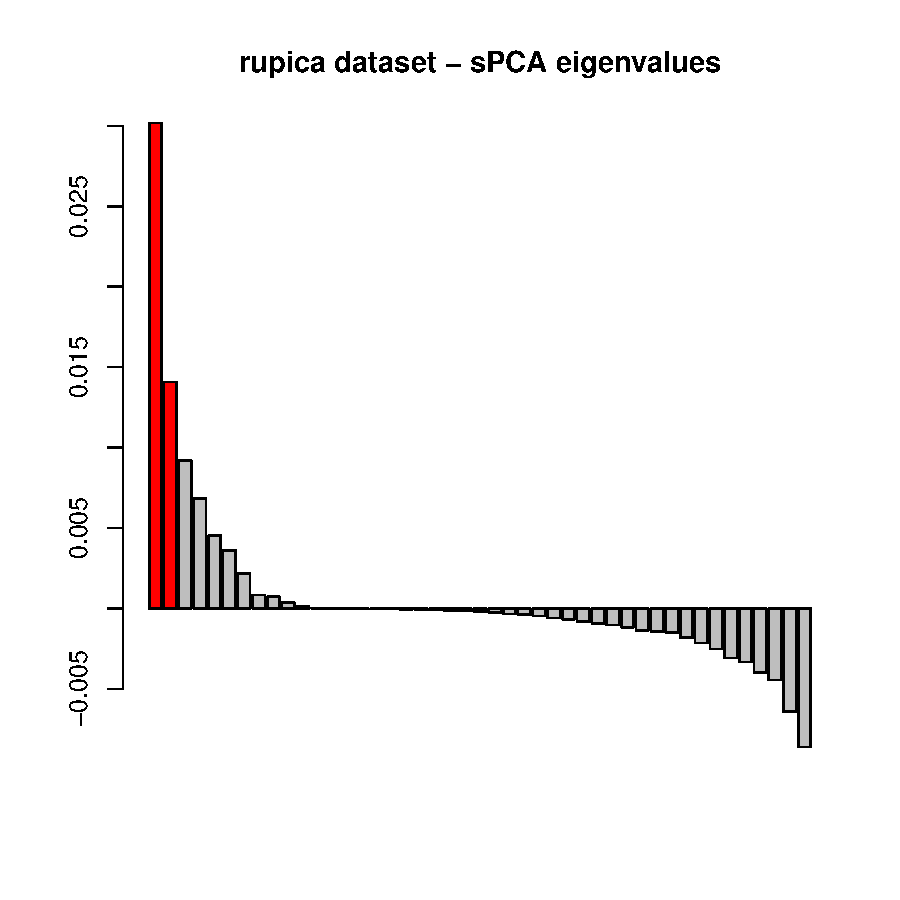
\includegraphics{figs/spca-048}

\noindent The principal components associated with the first two
positive eigenvalues (in red) shall be retained.
The printing of \texttt{spca} objects is more explicit than
\texttt{dudi} objects, but named with the same conventions:
\begin{Schunk}
\begin{Sinput}
> rupica.spca1
\end{Sinput}
\begin{Soutput}
	########################################
	# spatial Principal Component Analysis #
	########################################
class: spca
$call: spca(obj = rupica, cn = rupica.graph, scannf = FALSE, nfposi = 2, 
    nfnega = 0)

$nfposi: 2 axis-components saved
$nfnega: 0 axis-components saved
Positive eigenvalues: 0.03018 0.01408 0.009211 0.006835 0.004529 ...
Negative eigenvalues: -0.008611 -0.006414 -0.004451 -0.003963 -0.003329 ...

  vector length mode    content    
1 $eig   45     numeric eigenvalues

  data.frame nrow ncol content                                                 
1 $c1        55   2    principal axes: scaled vectors of alleles loadings      
2 $li        335  2    principal components: coordinates of entities ('scores')
3 $ls        335  2    lag vector of principal components                      
4 $as        2    2    pca axes onto spca axes                                 

$xy: matrix of spatial coordinates
$lw: a list of spatial weights (class 'listw')

other elements: NULL
\end{Soutput}
\end{Schunk}

Unlike usual multivariate analyses, eigenvalues of sPCA are composite:
they measure both the genetic diversity (variance) and the spatial
structure (spatial autocorrelation measured by Moran's $I$).
This decomposition can also be used to choose which principal
component to interprete.
The function \texttt{screeplot} allows to display this information graphically:
\begin{Schunk}
\begin{Sinput}
> screeplot(rupica.spca1)
\end{Sinput}
\end{Schunk}
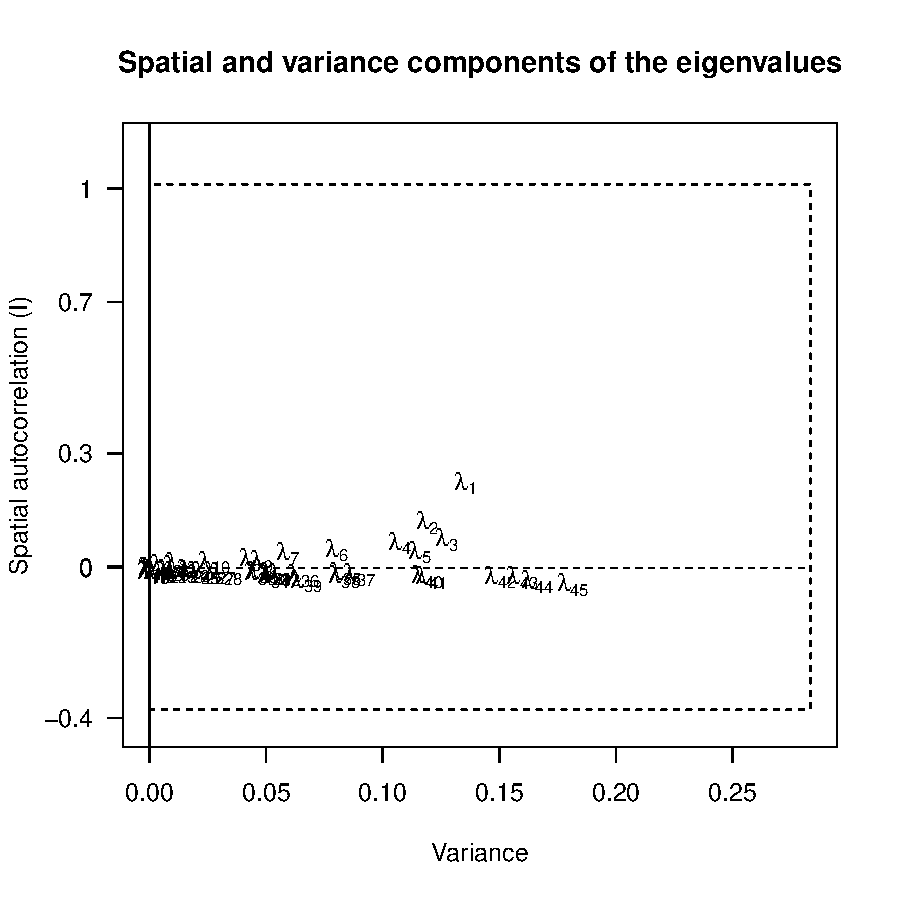
\includegraphics{figs/spca-050}

\noindent While $\lambda_1$ indicates with no doubt a structure, the
second eigenvalue, $\lambda_2$ is less clearly distinct from the
successive values.
Thus, we shall keep in mind this uncertainty when interpreting the
second principal component of the analysis.
\\


We map the sPCA results using \texttt{s.value} and lagged scores (\texttt{\$ls}) instead of the PC (\texttt{\$li}), which are a
'denoisified' version of the PCs.
\begin{Schunk}
\begin{Sinput}
> showBauges()
> s.value(rupica$other$xy, rupica.spca1$ls[, 1], add.p = TRUE, 
+     csize = 0.7)
> title("sPCA - first PC", col.main = "yellow", line = -2, cex.main = 2)
\end{Sinput}
\end{Schunk}
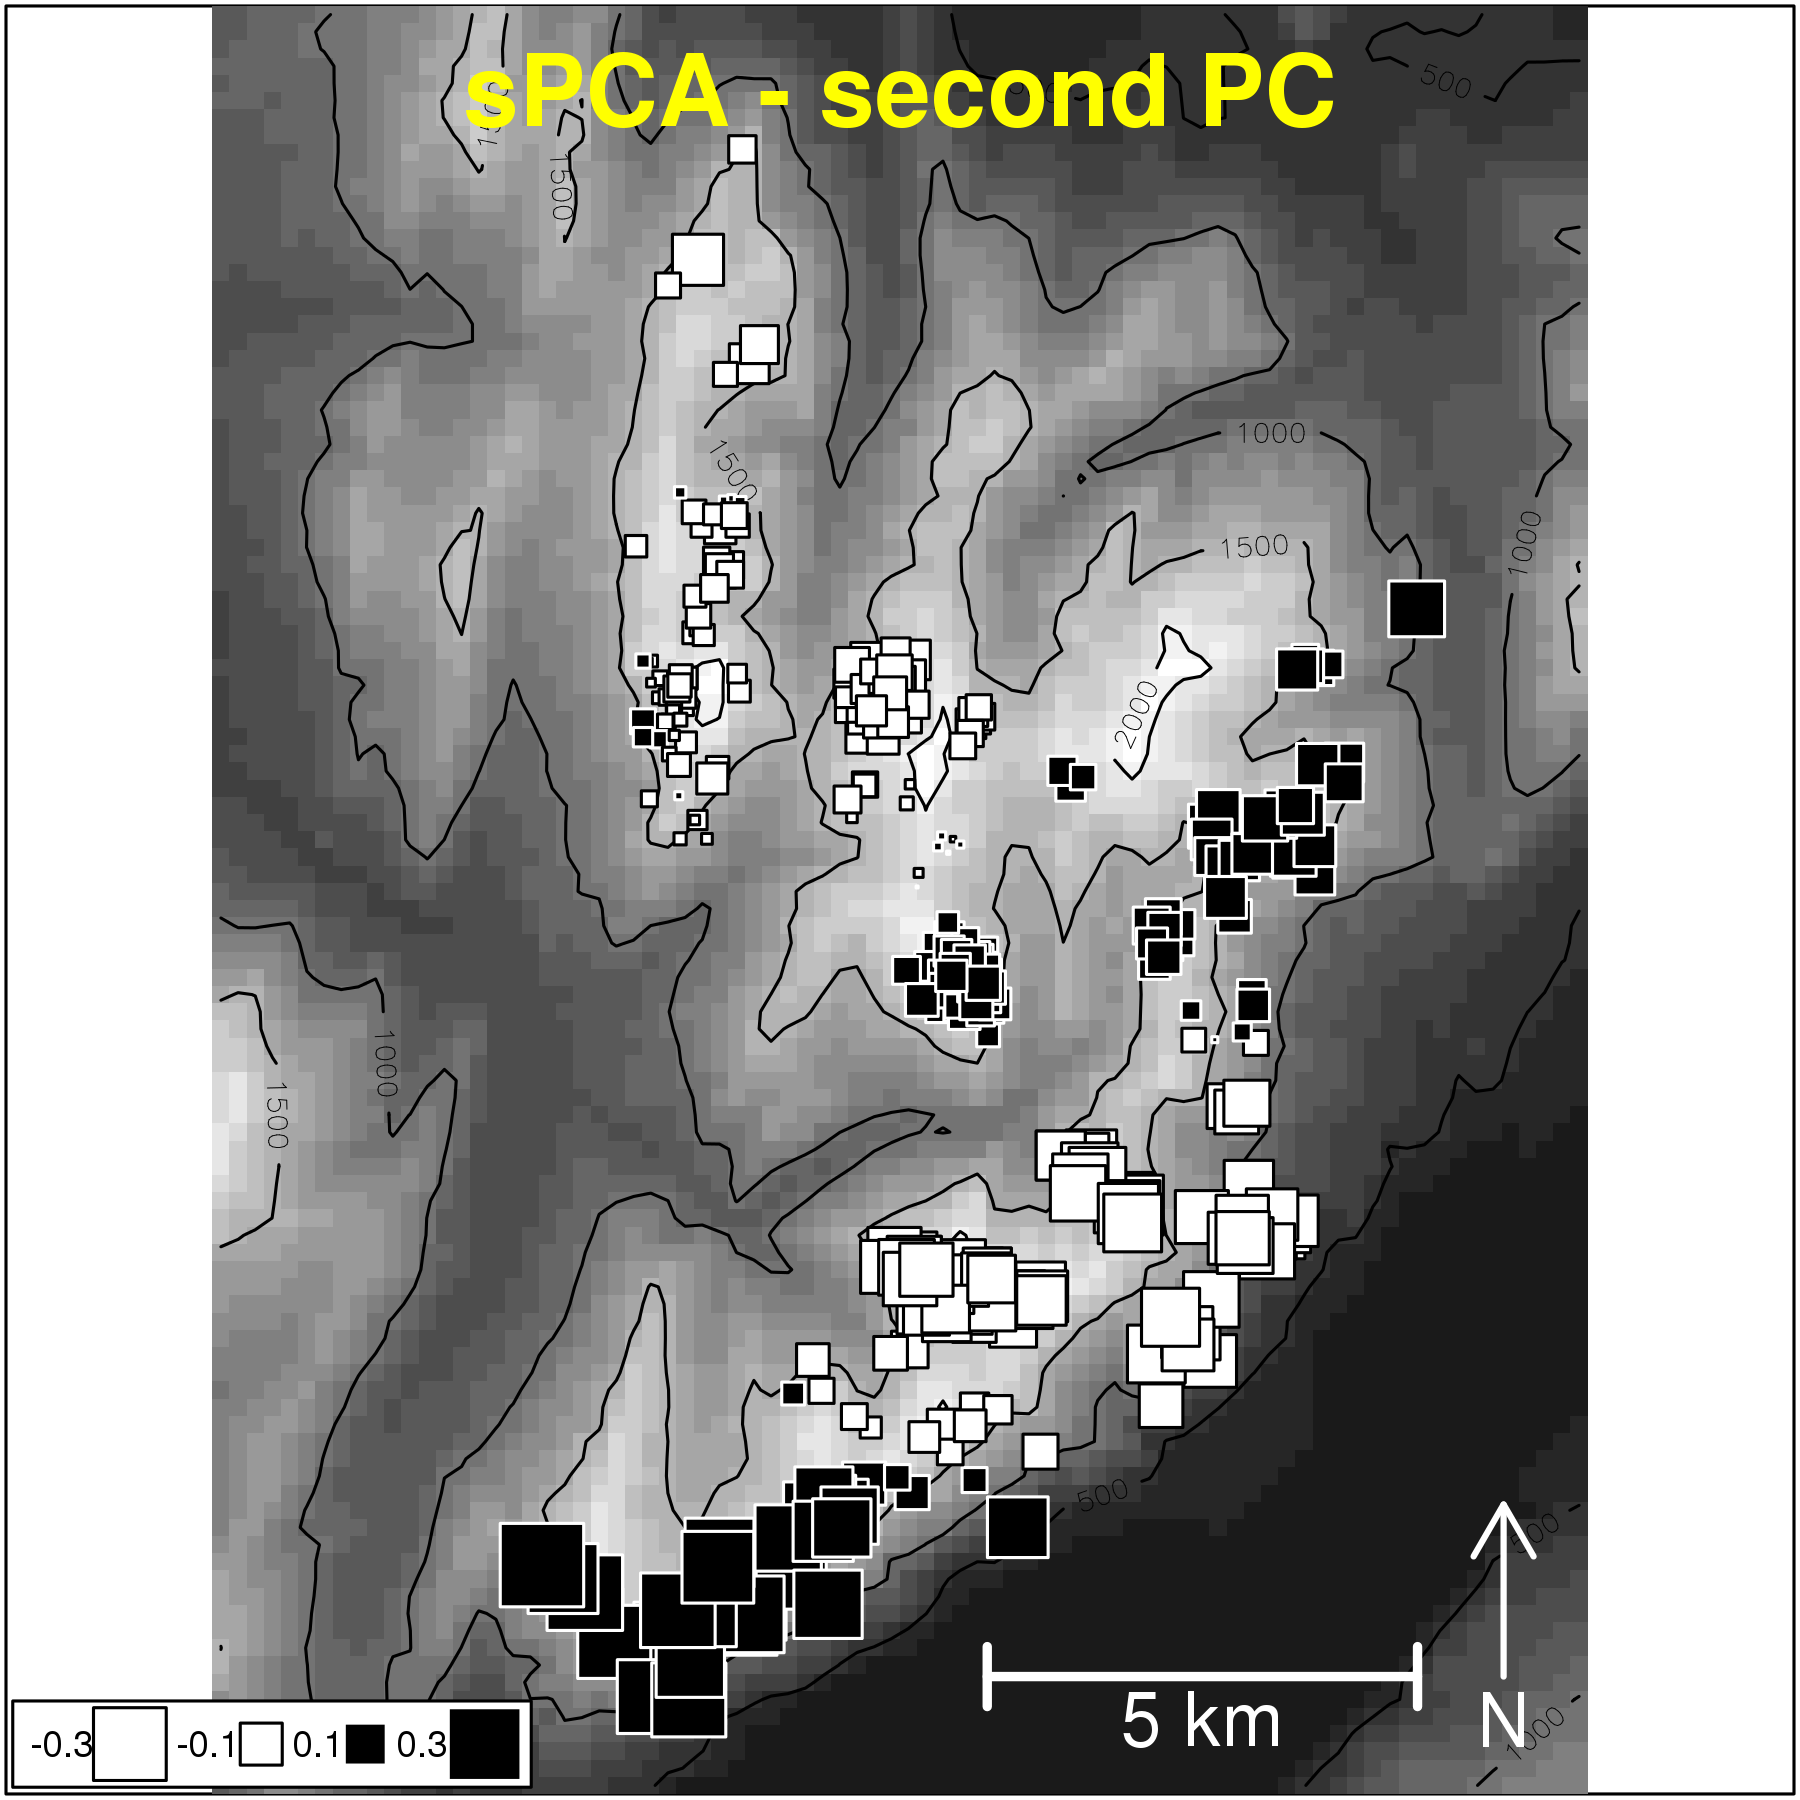
\includegraphics{figs/spca-051}

\noindent This first PC shows a remarkably clear structure opposing two high-altitude areas
separated by a valley, which is thought to be an obstacle to the dispersal of Chamois (due to higher
exposition to predation in low-altitude areas).

The second PC of sPCA shows an equally interesting structure:
\begin{Schunk}
\begin{Sinput}
> showBauges()
> s.value(rupica$other$xy, rupica.spca1$ls[, 2], add.p = TRUE, 
+     csize = 0.7)
> title("sPCA - second PC", col.main = "yellow", line = -2, cex.main = 2)
\end{Sinput}
\end{Schunk}
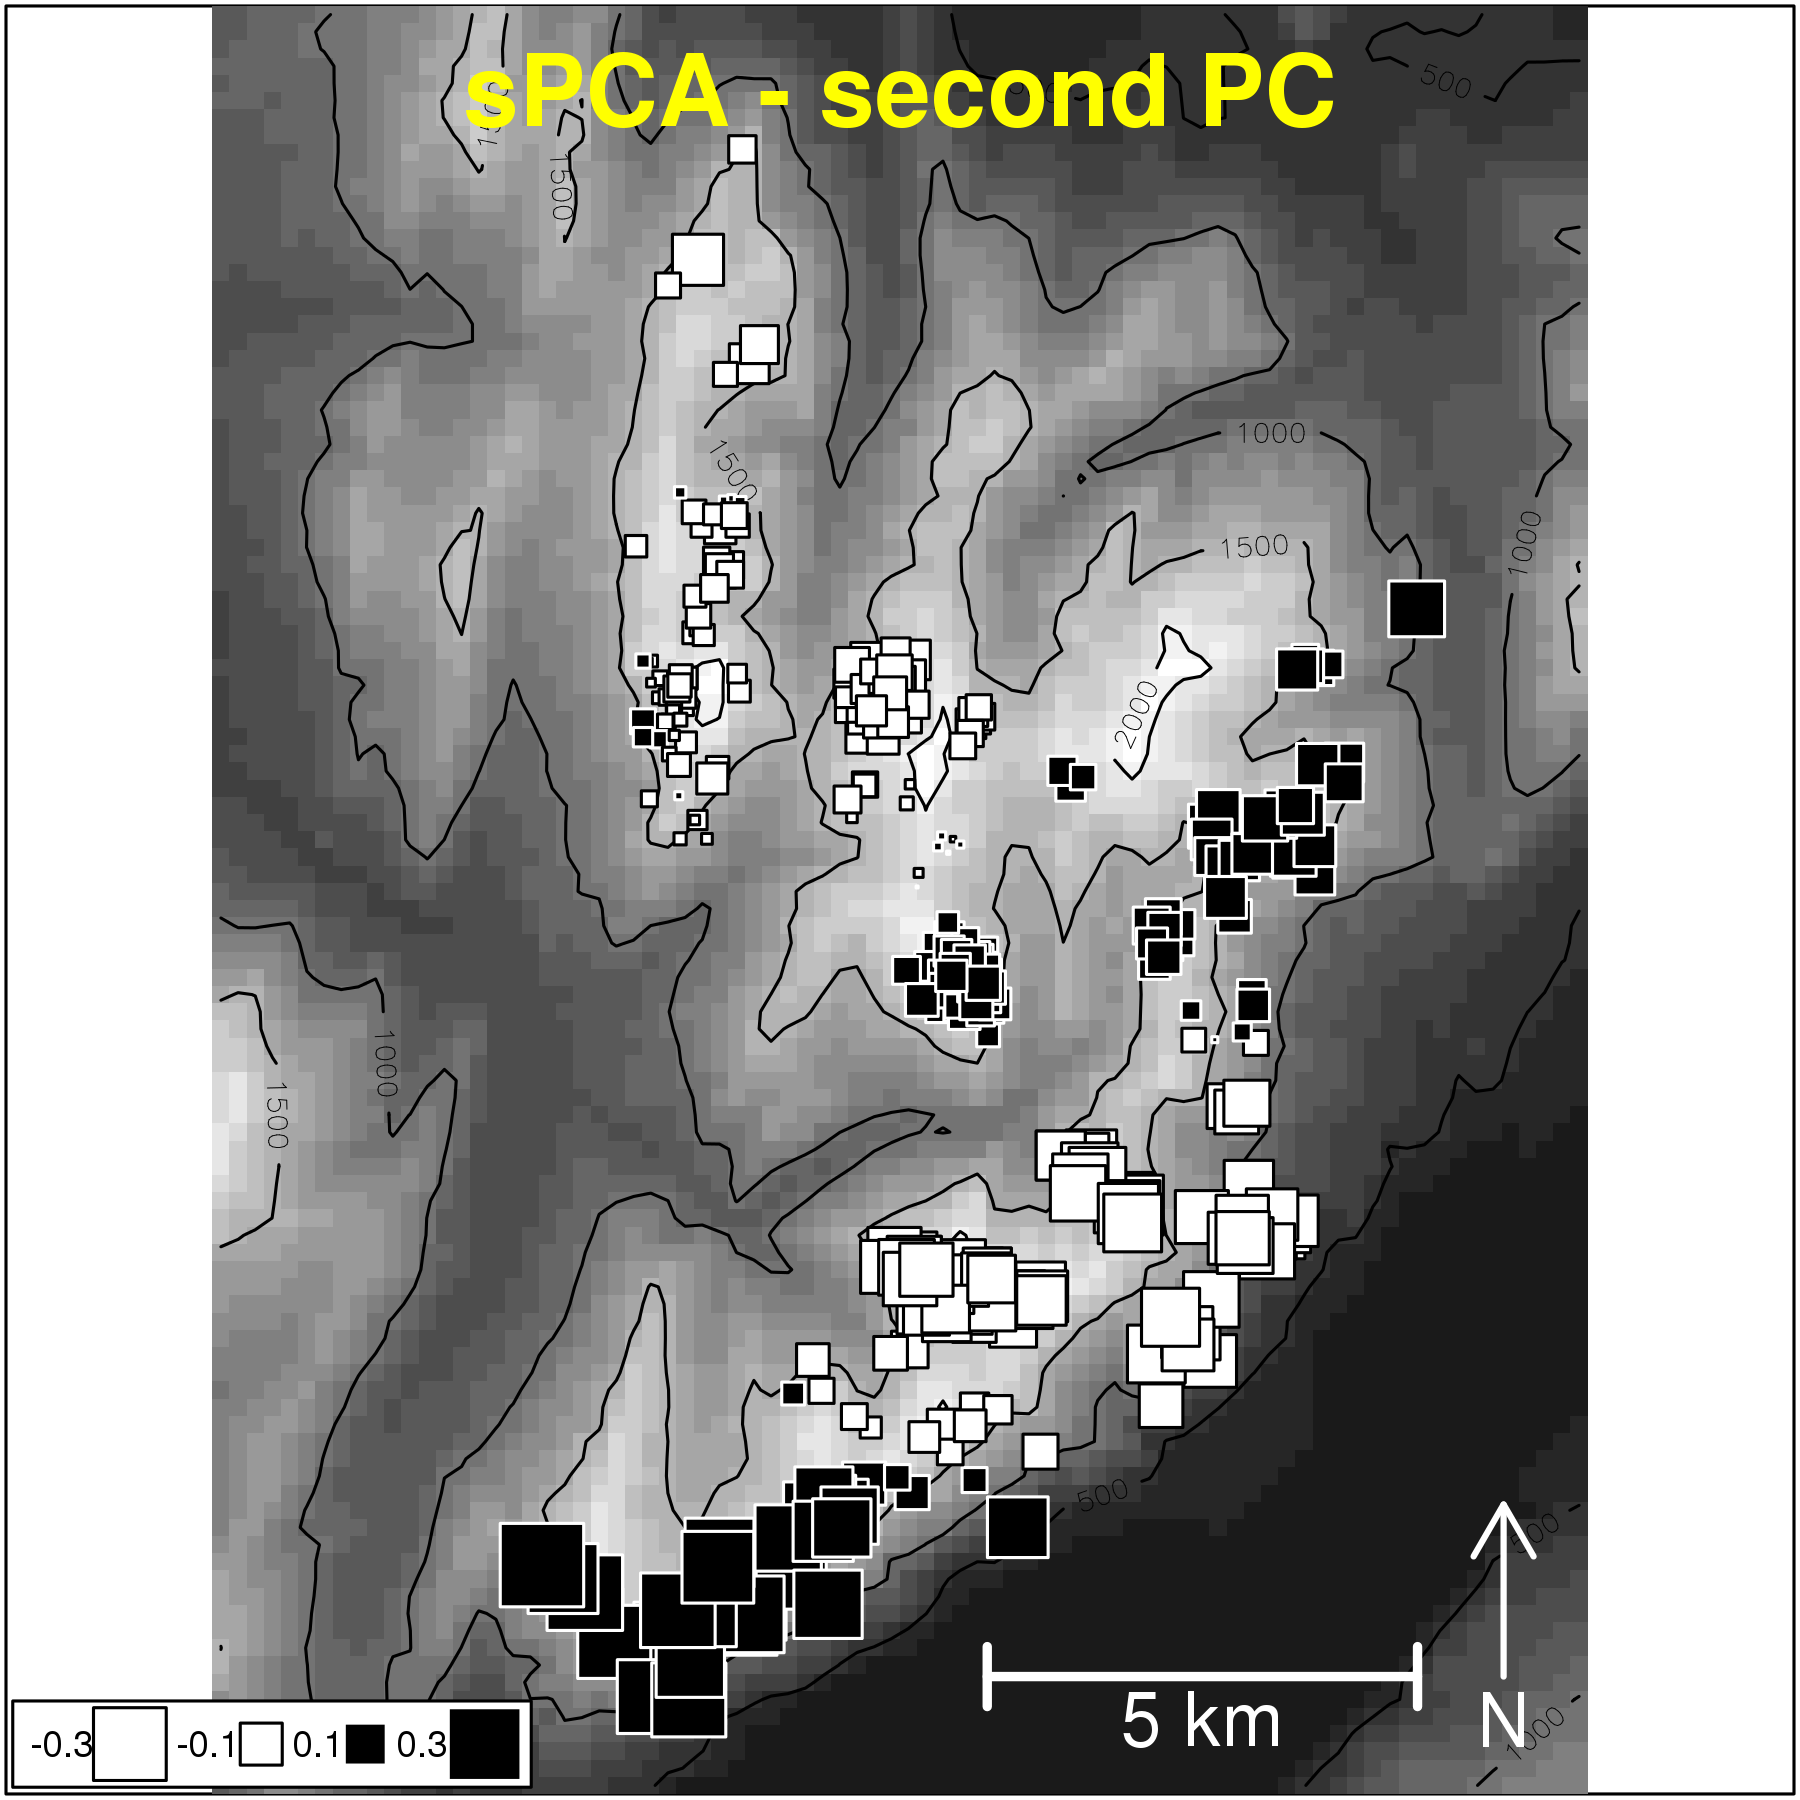
\includegraphics{figs/spca-052}

\noindent The smaller clusters appearing on this map correspond to social units identified by
direct observation in the field.
Therefore, this genetic structure is merely a reflect of the social behaviour of these individuals.
\\


Both genetic structures can be represented altogether using \texttt{colorplot}.
The final figure should ressemble this (although colors may change from one computer to another):
\begin{Schunk}
\begin{Sinput}
> showBauges()
> colorplot(rupica$other$xy, rupica.spca1$ls, axes = 1:2, transp = TRUE, 
+     add = TRUE, cex = 3)
> title("sPCA - colorplot of PC 1 and 2\n(lagged scores)", col.main = "yellow", 
+     line = -2, cex = 2)
\end{Sinput}
\end{Schunk}
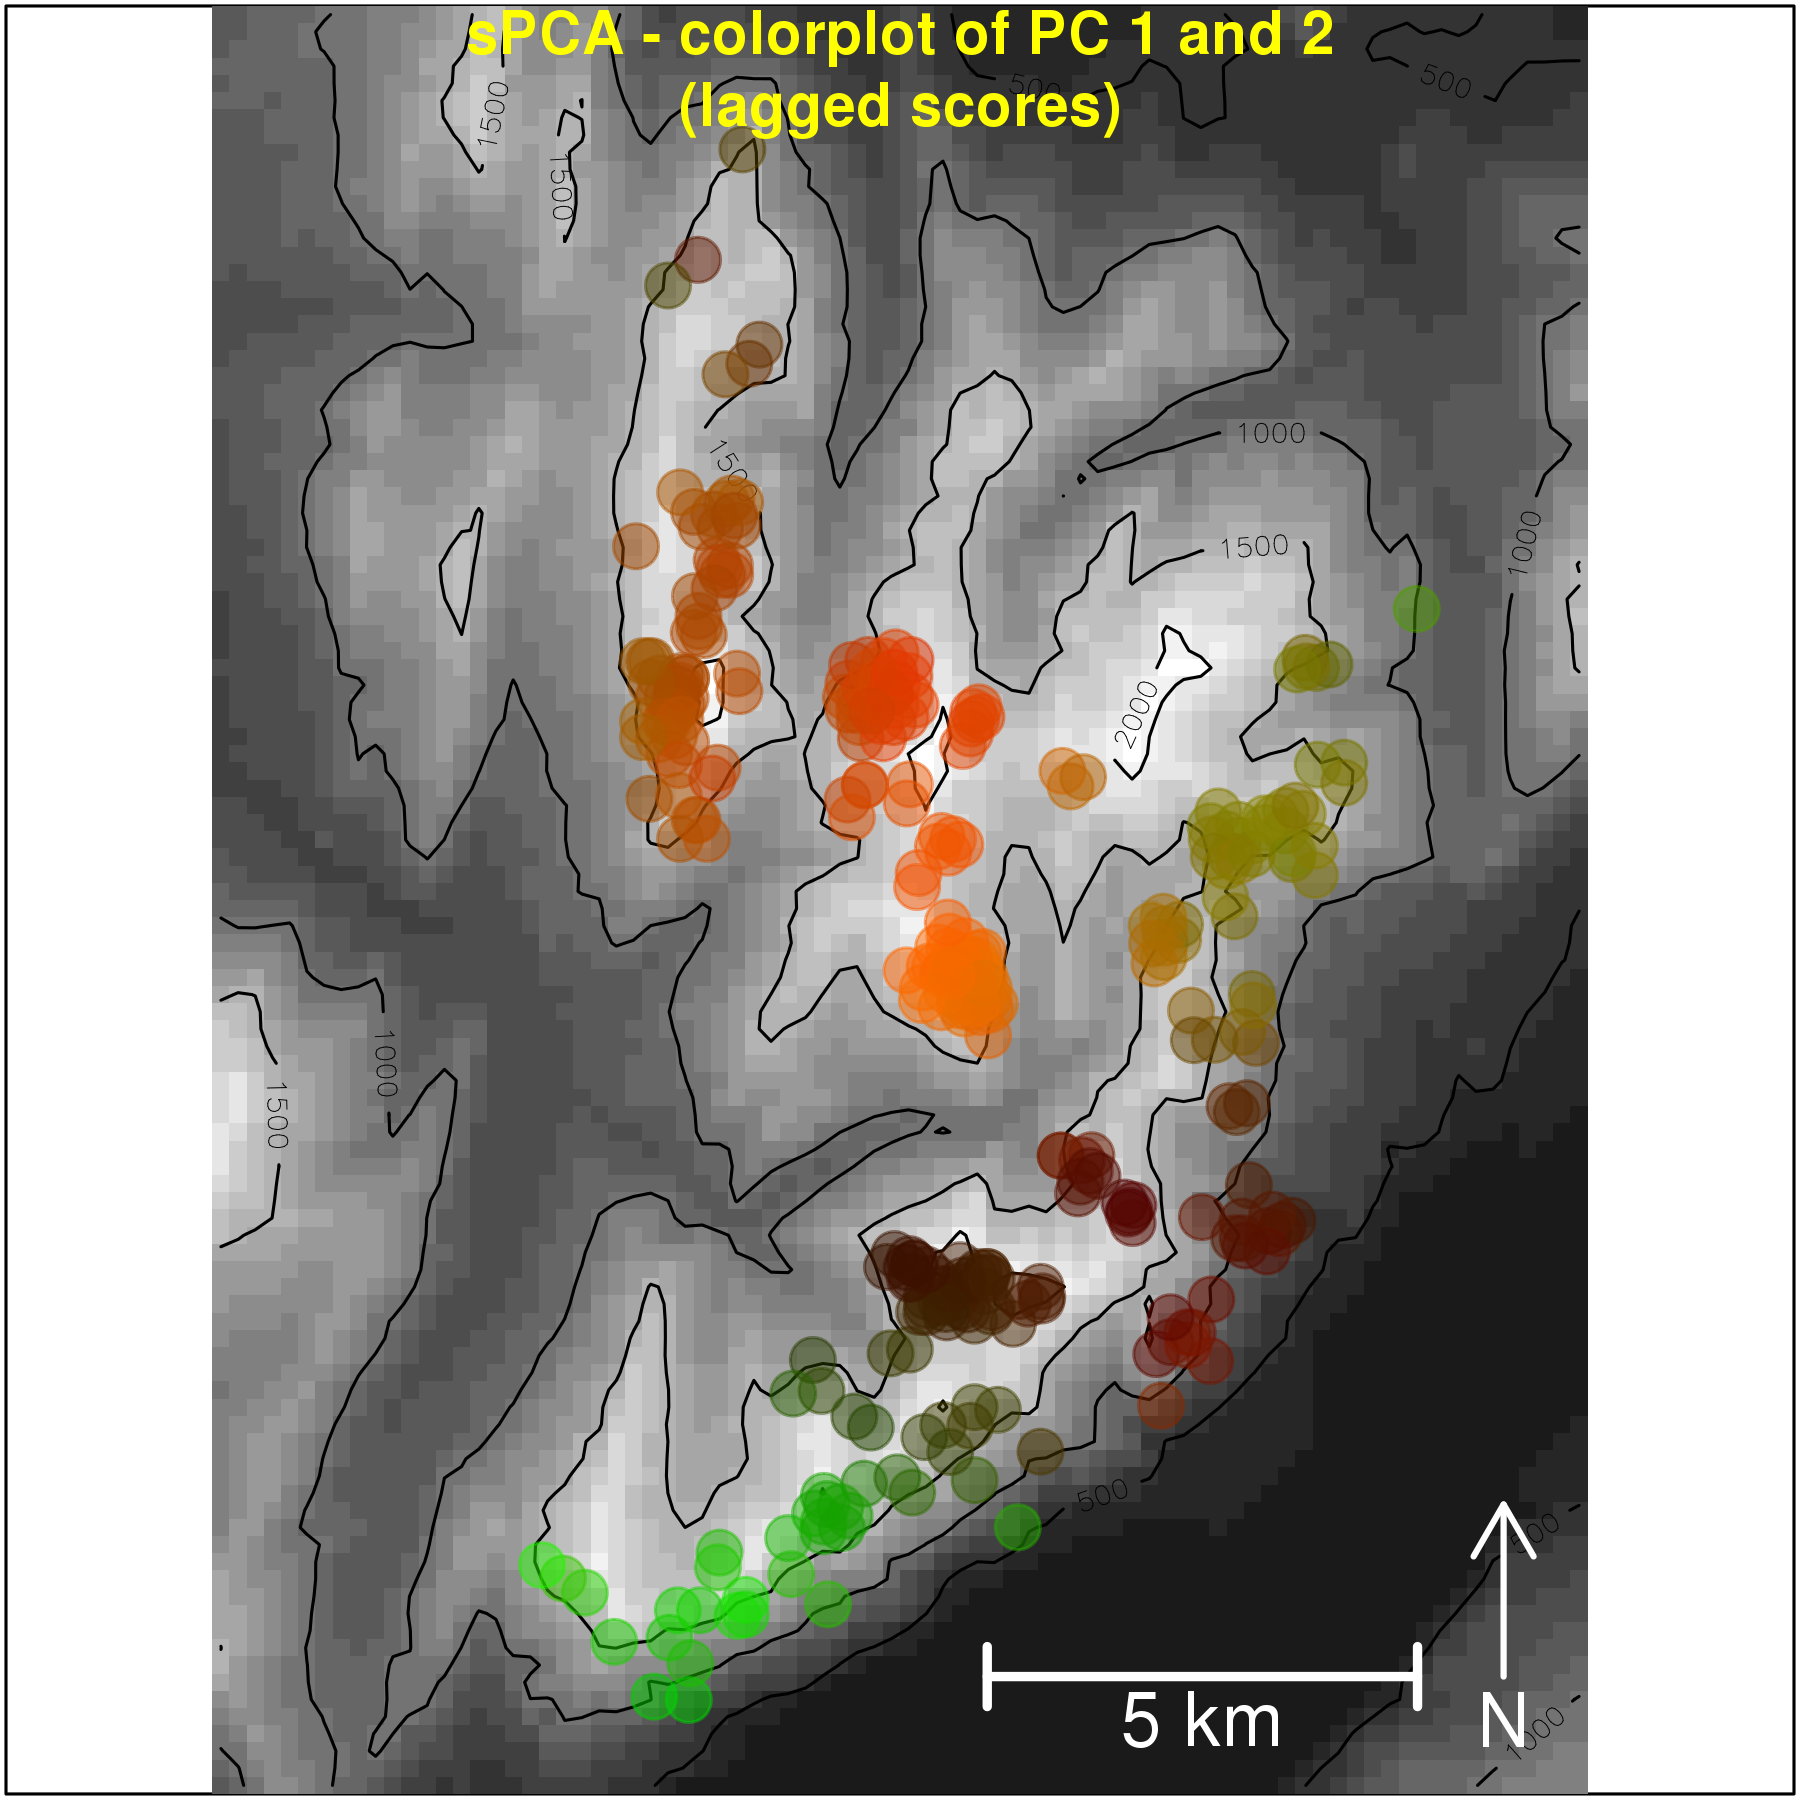
\includegraphics{figs/spca-053}

%% \begin{center}
%% 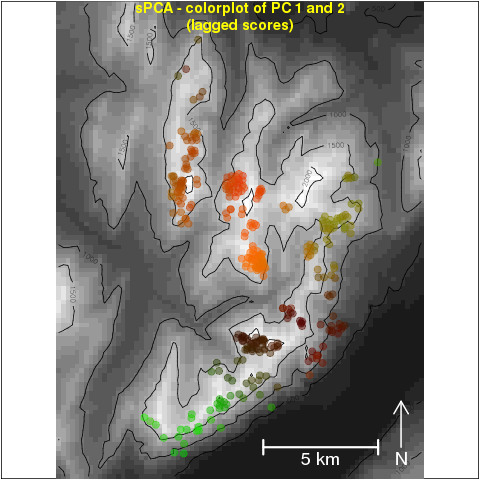
\includegraphics[width=.6\textwidth]{figs/rupicacolors.png}
%% \end{center}






\newpage
\begin{thebibliography}{9}

\bibitem{tjart04}
  Jombart T, Devillard S, Dufour A-B and Pontier D (2008) Revealing cryptic spatial
  patterns in genetic variability by a new multivariate method.  \textit{Heredity} 101: 92-103.

\bibitem{tjart05}
  Jombart, T. (2008) adegenet: a R package for the multivariate
  analysis of genetic markers. \textit{Bioinformatics} 24: 1403-1405.

\bibitem{np145}
  R Development Core Team (2011) R: A language and environment for
  statistical computing. R Foundation for Statistical Computing,
  Vienna, Austria. ISBN 3-900051-07-0.

%% \bibitem{tj548}
%%   Dray S and Dufour A-B (2007) The ade4 package: implementing the duality diagram for ecologists. \textit{Journal of Statistical Software} 22: 1-20.

%% \bibitem{tjart19}
%%   Jombart T, Devillard S and Balloux, F (2010).
%%   Discriminant analysis of principal components: a new method for the analysis of genetically structured populations.
%%   \textit{BMC Genetics} 11: 94.


\bibitem{tj88}
  Legendre P and Legendre L (1998) Numerical ecology. Elsevier Science B. V., Amsterdam.

\bibitem{tj223}
  Moran P (1948). The interpretation of statistical maps.
  \emph{Journal of the Royal Statistical Society, B} 10: 243--251.

\bibitem{tj222}
  Moran, P. (1950) Notes on continuous stochastic phenomena. \emph{Biometrika} 37: 17--23.

\bibitem{tj436} Cliff A and Ord J (1981) \emph{Spatial Processes. Model \& Applications}. London: Pion.

\bibitem{tj179} Menozzi P, Piazza A and Cavalli-Sforza LL (1978) Synthetic maps of human gene frequencies in {Europeans}.
  \emph{Science} 201: 786--792.

%% \bibitem{tj177}
%% Cavalli-Sforza LL, Menozzi P and Piazza A (1993) Demic expansions and human evolution.
%%  \textit{Science} 259: 639--646.

\bibitem{tj440}
  Callenge C (2006) The package "adehabitat" for the R software: a tool for the analysis
  of space and habitat use by animals. \textit{Ecological Modelling} 197: 516--519.


%% \bibitem{tjart20}
%%   Jombart T, Eggo RM, Dodd PJ and Balloux F (2010) Reconstructing disease outbreaks from genetic
%%   data: a graph approach. \textit{Heredity} 106: 383-390.

%% \bibitem{tjart10}
%%   Jombart T, Pontier D and Dufour A-B (2009) Genetic markers in the playground of multivariate analysis.
%%   \textit{Heredity} 102: 330-341.

%% \bibitem{tj527}
%%   Paradis E, Claude J, and Strimmer K (2004) APE: analyses of phylogenetics and evolution in R language.
%%   \textit{Bioinformatics}: 20, 289-290.

%% \bibitem{np160}
%%   Charif D, and Lobry J (2007) SeqinR 1.0-2: a contributed package to the R project for statistical
%%   computing devoted to biological sequences retrieval and analysis. \textit{in} Structural approaches to sequence evolution: Molecules, networks, populations, \textit{Springer Verlag}, 207-232.

%% \bibitem{tj814}
%%   Nei M (1973) Analysis of gene diversity in subdivided populations. \textit{Proc Natl Acad Sci USA} 70: 3321-3323.


%% \bibitem{tj433}
%%   Monmonier M (1973) Maximum-difference barriers: an alternative numerical regionalization method. \textit{Geographical Analysis} 3: 245-261.

%% \bibitem{np120}
%%   Manni F, Guerard E and Heyer E (2004) Geographic patterns of (genetic, morphologic, linguistic)
%%   variation: how barriers can be detected by "Monmonier's algorithm". \textit{Human Biology} 76: 173-190.


\end{thebibliography}

\end{document}

